% CHAPITRE 4
\singlespacing
\chapter{Effets de l'hydrologie sur les flux de GES -- approche expérimentale}
\label{ch:4}

\minitoc

\newpage
\doublespacing
%\section{Manipulation du niveau de l'eau en mésocosmes}
\section{Introduction}


% de cette faible variation peu de variations des flux ont pu y être relié.
L'hydrologie est reconnue comme un facteur contrôlant les flux de GES \citep{blodau2002}.
En effet de nombreuses études ont relié les émissions de \coo au niveau de la nappe d'eau (Tableau~\ref{table:bib_wtl}).
La majorité d'entre elles montrent qu'une tourbière dont le niveau de la nappe est abaissé, soit par un drainage, soit par une sécheresse, a un ENE plus faible.
Cependant, aucun consensus n'a encore été atteint concernant les origines de ces baisses de l'ENE.
\citet{strack2013} expliquent ainsi le fonctionnement en source de carbone d'une tourbière Canadienne par des conditions plus chaudes et plus sèches que les moyennes observées à plus long terme sur le site.
Une observation similaire est faite par \citet{aurela2007} qui mesurent un ENE plus faible lors d'une année sèche, dans une tourbière à Carex au sud de la Finlande.
Ils attribuent également cette baisse de l'ENE aux conditions plus chaudes et plus sèches, qui permettent le développement d'une zone aérobie plus importante et favorise ainsi une RE plus élevée.
Lors d'un suivi de douze années sur une tourbière Suédoise, \citet{peichl2014} observent également une baisse de l'ENE lors d'une année ou le niveau de la nappe baisse de façon importante, en dessous de \SI{-30}{\centi\metre} de profondeur.

%Ils attribuent la variation de l'ENE aux conditions plus chaudes et sèches qui, principalement, augmentent la RE (effet de la température sur les vitesses de réaction et développement d'une zone aérobie permettant la respiration plus importante) et diminuent légèrement la PPB (suite à un stress hydrique de la végétation).
%Ils attribuent la variation de l'ENE majoritairement à une augmentation de la RE et à une légère baisse de la PPB (liée à un stress hydrique), dans des conditions plus chaudes et plus sèches.
%\citet{peichl2014} observent également une baisse de l'ENE lors d'une année ou le niveau de la nappe baisse de façon importante, en dessous de \SI{-30}{\centi\metre} de profondeur.
Ils expliquent cette baisse par une baisse de la PPB.
Cette observation va dans le même sens que celles de \citet{lund2012} sur un suivi de quatre années (2006--2009) dans une tourbière à sphaignes située au sud de la Suède. 
Dans cette étude, ils observent deux années de sécheresse, 2006 et 2008, pour lesquelles l'ENE est plus faible que la moyenne.
En 2006 ils observent également des valeurs de RE plus importantes que les autres années, ce qui explique l'ENE faible observée.
En revanche en 2008, ce n'est pas par la RE qu'ils expliquent les valeurs de l'ENE, mais par la PPB qui est plus faible cette année là.
Dans les deux cas la baisse du niveau de l'eau conduit à une baisse de l'ENE, cependant cette baisse a des origines différentes.
Les auteurs expliquent ces différences par le type de sécheresse : courte et intense pendant la saison de végétation de 2006 et d'intensité plus faible mais d'une durée plus longue en 2008.
%Ces inconsistances apparentes peuvent avoir pour origine des types de sécheresse différentes : courte et intense pendant la saison de végétation de 2006 et d'intensité plus faible mais d'une durée plus longue en 2008.
À l'inverse des résultats précédemment cités, \citet{ballantyne2014} dans une étude sur les effets à long terme d'une baisse du niveau de la nappe, n'observent pas d'effets significatifs sur l'ENE tandis que les flux de RE et de PPB augmentent tous les deux.
Ces études montrent que si le niveau de la nappe est reconnu comme un facteur de contrôle des flux de \coo, il est difficile d'en dégager des liens de cause à effet répétables.

\begin{table}
\centering
\caption{Effet d'une baisse du niveau de la nappe d'eau (asséchement) dans les tourbières sur les flux de \coo. Les flèches rouges montantes décrivent une augmentation du flux et les flèches bleues une diminution.}
\label{table:bib_wtl}
\begin{tabular}{llll}\toprule
Référence & ENE & RE & PPB \\ \midrule
\citealp{strack2013}& \decarrow & \incarrow & \decarrow \\ 
\citealp{aurela2007} & \decarrow & \incarrow & NA \\ 
\citealp{peichl2014} & \decarrow & $\rightarrow$ & \decarrow \\ 
%	Sonnentag \textit{et al}., 2010 & \decarrow &  T  & \decarrow \\ 
%	\addlinespace[.15cm]
\citealp{lund2012} & \decarrow & \incarrow & $\rightarrow$ \\
\citealp{lund2012} & \decarrow & $\rightarrow$ & \decarrow \\
\citealp{ballantyne2014} & $\rightarrow$ & \incarrow & \incarrow \\ 

\bottomrule
\end{tabular}
\end{table}


Concernant de \chh, un niveau de nappe d'eau haut est généralement associé à des émissions importantes et un niveau de nappe bas à des émissions faibles.
Ceci est lié au fait que le niveau de la nappe d'eau contrôle l'épaisseur de la zone où le \chh est produit ainsi que celle ou il est oxydé \citep{pelletier2007}.
%Concernant le \chh, une baisse du niveau de la nappe d'eau est généralement liée à une baisse des émissions, et inversement.
%Ceci provient du fait que le niveau de la nappe d'eau contrôle l'épaisseur de la zone où le \chh est produit/oxydé \citep{pelletier2007}.
\citet{turetsky2008} montrent que l'effet des variations du niveau de nappe sur les flux de \chh n'est pas répétable.
Ils observent également que l'effet sur les flux de \chh est plus important lorsque le niveau de la nappe est augmenté que lorsqu'il est diminué ($\pm$ \SI{10}{\centi\metre}).
Pour expliquer cette observation, ils font l'hypothèse que, lorsque le niveau de la nappe d'eau est plus élevé, le transfert de chaleur dans le sol est plus rapide et permet de maintenir des températures plus élevées qui favorisent la production de \chh.
%Ils font l'hypothèse que le niveau de la nappe, en plus d'agir sur la proportion production/oxydation du \chh, a un effet sur le transfert de chaleur dans le sol.
%Cette hypothèse s'appuie sur l'observation de températures plus élevées, que ce soit celles de l'air ou de la tourbe, dans les zones où le niveau de la nappe a été rehaussé.
Cependant d'autres études, principalement dans des sites où le niveau de la nappe est proche de la surface du sol, montrent une absence de relation entre le niveau de la nappe et les émissions de \chh, voire une relation inverse, avec des flux plus faibles liés à des niveaux de nappe plus élevés \citep{kettunen1996,bellisario1999,treat2007}.
Pour expliquer ces observations, l'hypothèse avancée est que le \chh est piégé dans une porosité du sol fermée par la saturation importante en eau.
%L'hypothèse avancée pour expliquer ces observations explique que le \chh est immobilisé dans la porosité du sol 
%L'explication avancée étant un bloquage du \chh dans la porosité saturée en eau
Là encore selon les conditions environnementales, la relation entre les flux de \chh et le niveau de la nappe n'est pas aisément généralisable.

Lors d'expérimentations consistant à manipuler le niveau de la nappe d'eau, la vitesse et/ou la manière de simuler une remontée du niveau de l'eau peut également influencer la réponse des flux de GES.
%La vitesse de l'augmentation du niveau de nappe semble également influencer les flux ; des pics de RE ayant été observés après une réhumectation rapide du sol.
%La manière de simuler la réhumectation influence également les flux.
%La façon dont le niveau de la nappe augmente semble également jouer sur les flux.
\citet{strack2009} ont ainsi observé en suivant les flux de \coo sur des mésocomes de tourbe, qu'une réhumectation graduelle alimentée par le bas de la colonne de sol conduisait à une baisse de la RE, alors qu'une hausse rapide par le haut de la colonne (simulant un événement pluvieux) conduisait à un pic de RE.
Une observation similaire d'augmentation importante de la RE après réhumectation a également été observée par  \citet{mcneil2003}.
%Cette hausse de la RE après une réhumectation a également été observé par \citet{mcneil2003}.


%L'objectif de ce chapitre est d'explorer plus en avant l'effet des variations du niveau de la nappe d'eau dans des mésocosmes, sur les émissions de GES.
Au cours des deux années de suivi des flux de \coo et de \chh dans la tourbière de La Guette (2013 et 2014), le niveau de la nappe d'eau est resté relativement élevé et a très faiblement varié en comparaison avec les années précédentes bien plus sèches (Figure~\ref{fig:WTL}).
En conséquence, l'effet des variations de nappe d'eau sur les flux de GES n'a pu être investigué.
L'effet de cycles de dessiccation/réhumectation sur les émissions de \coo et de \chh est cependant certain et on peut faire l'hypothèse qu'une baisse du niveau de la nappe entraînerait une augmentation des flux de RE, et possiblement une diminution des flux de \chh.
On peut également attendre un pic d'émission de la RE au moment de la réhumectation.

L'objectif de ce chapitre est donc de déterminer les effets de variations du niveau de la nappe sur les flux de GES à travers deux expérimentations simulant des phases de dessiccation et de réhumectation d'un sol tourbeux.

\section{Procédure expérimentale}

\begin{figure}
\centering
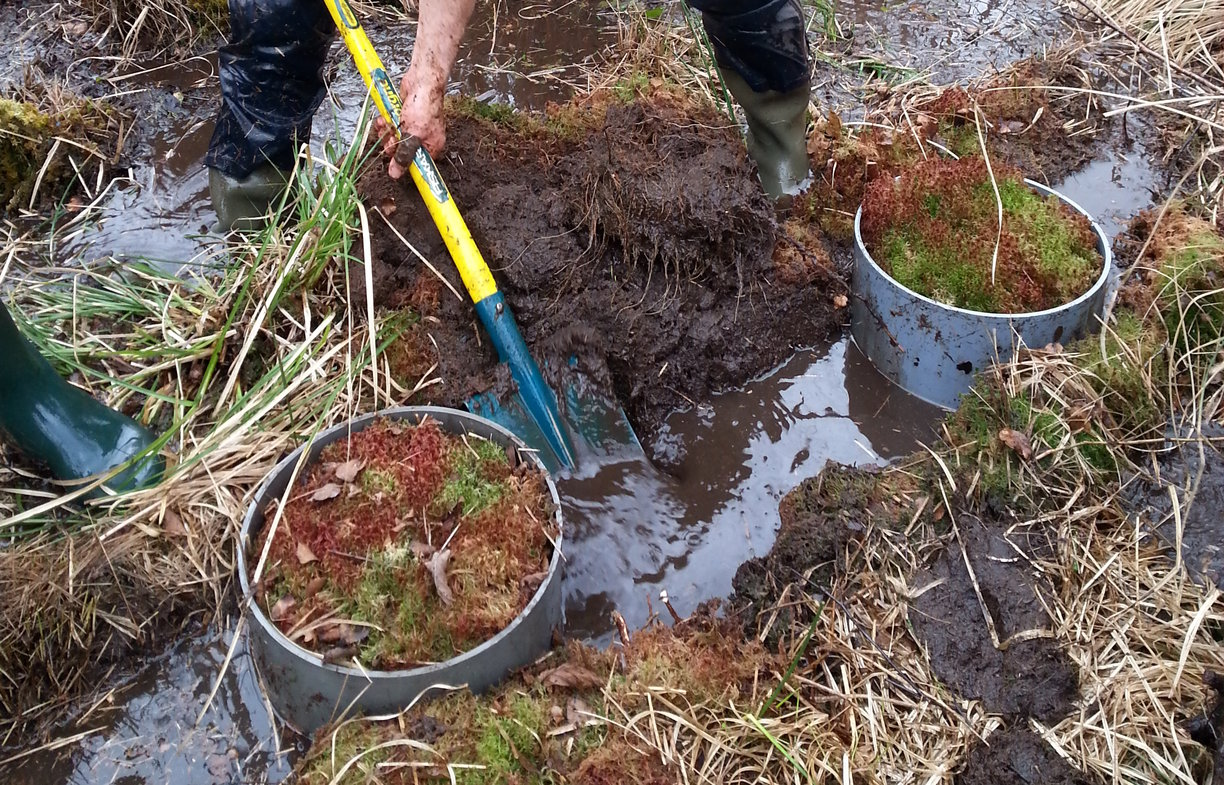
\includegraphics[width=\textwidth]{chap4/mesocosmes}\\
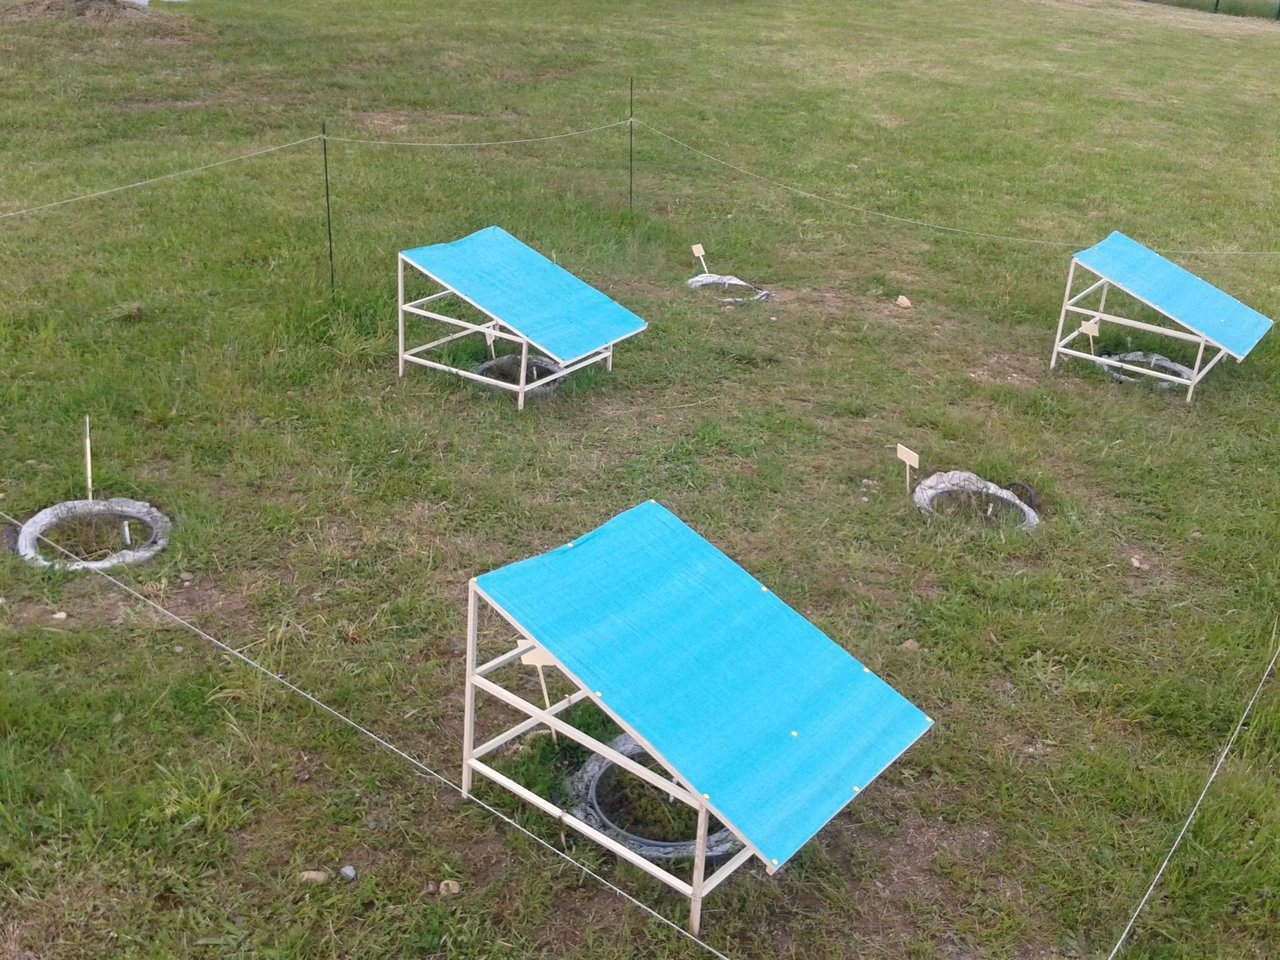
\includegraphics[width=\textwidth]{chap4/zi_exp_low}
\caption{Prélèvement des mésocosmes sur la tourbière de La Guette (en haut). Mésocosmes installés près du laboratoire : 6 témoins et 6 traités, avec des dispositifs pour intercepter la pluie (en bas).}
\label{fig:mesophoto}
\end{figure}


%\begin{figure}
%\centering
%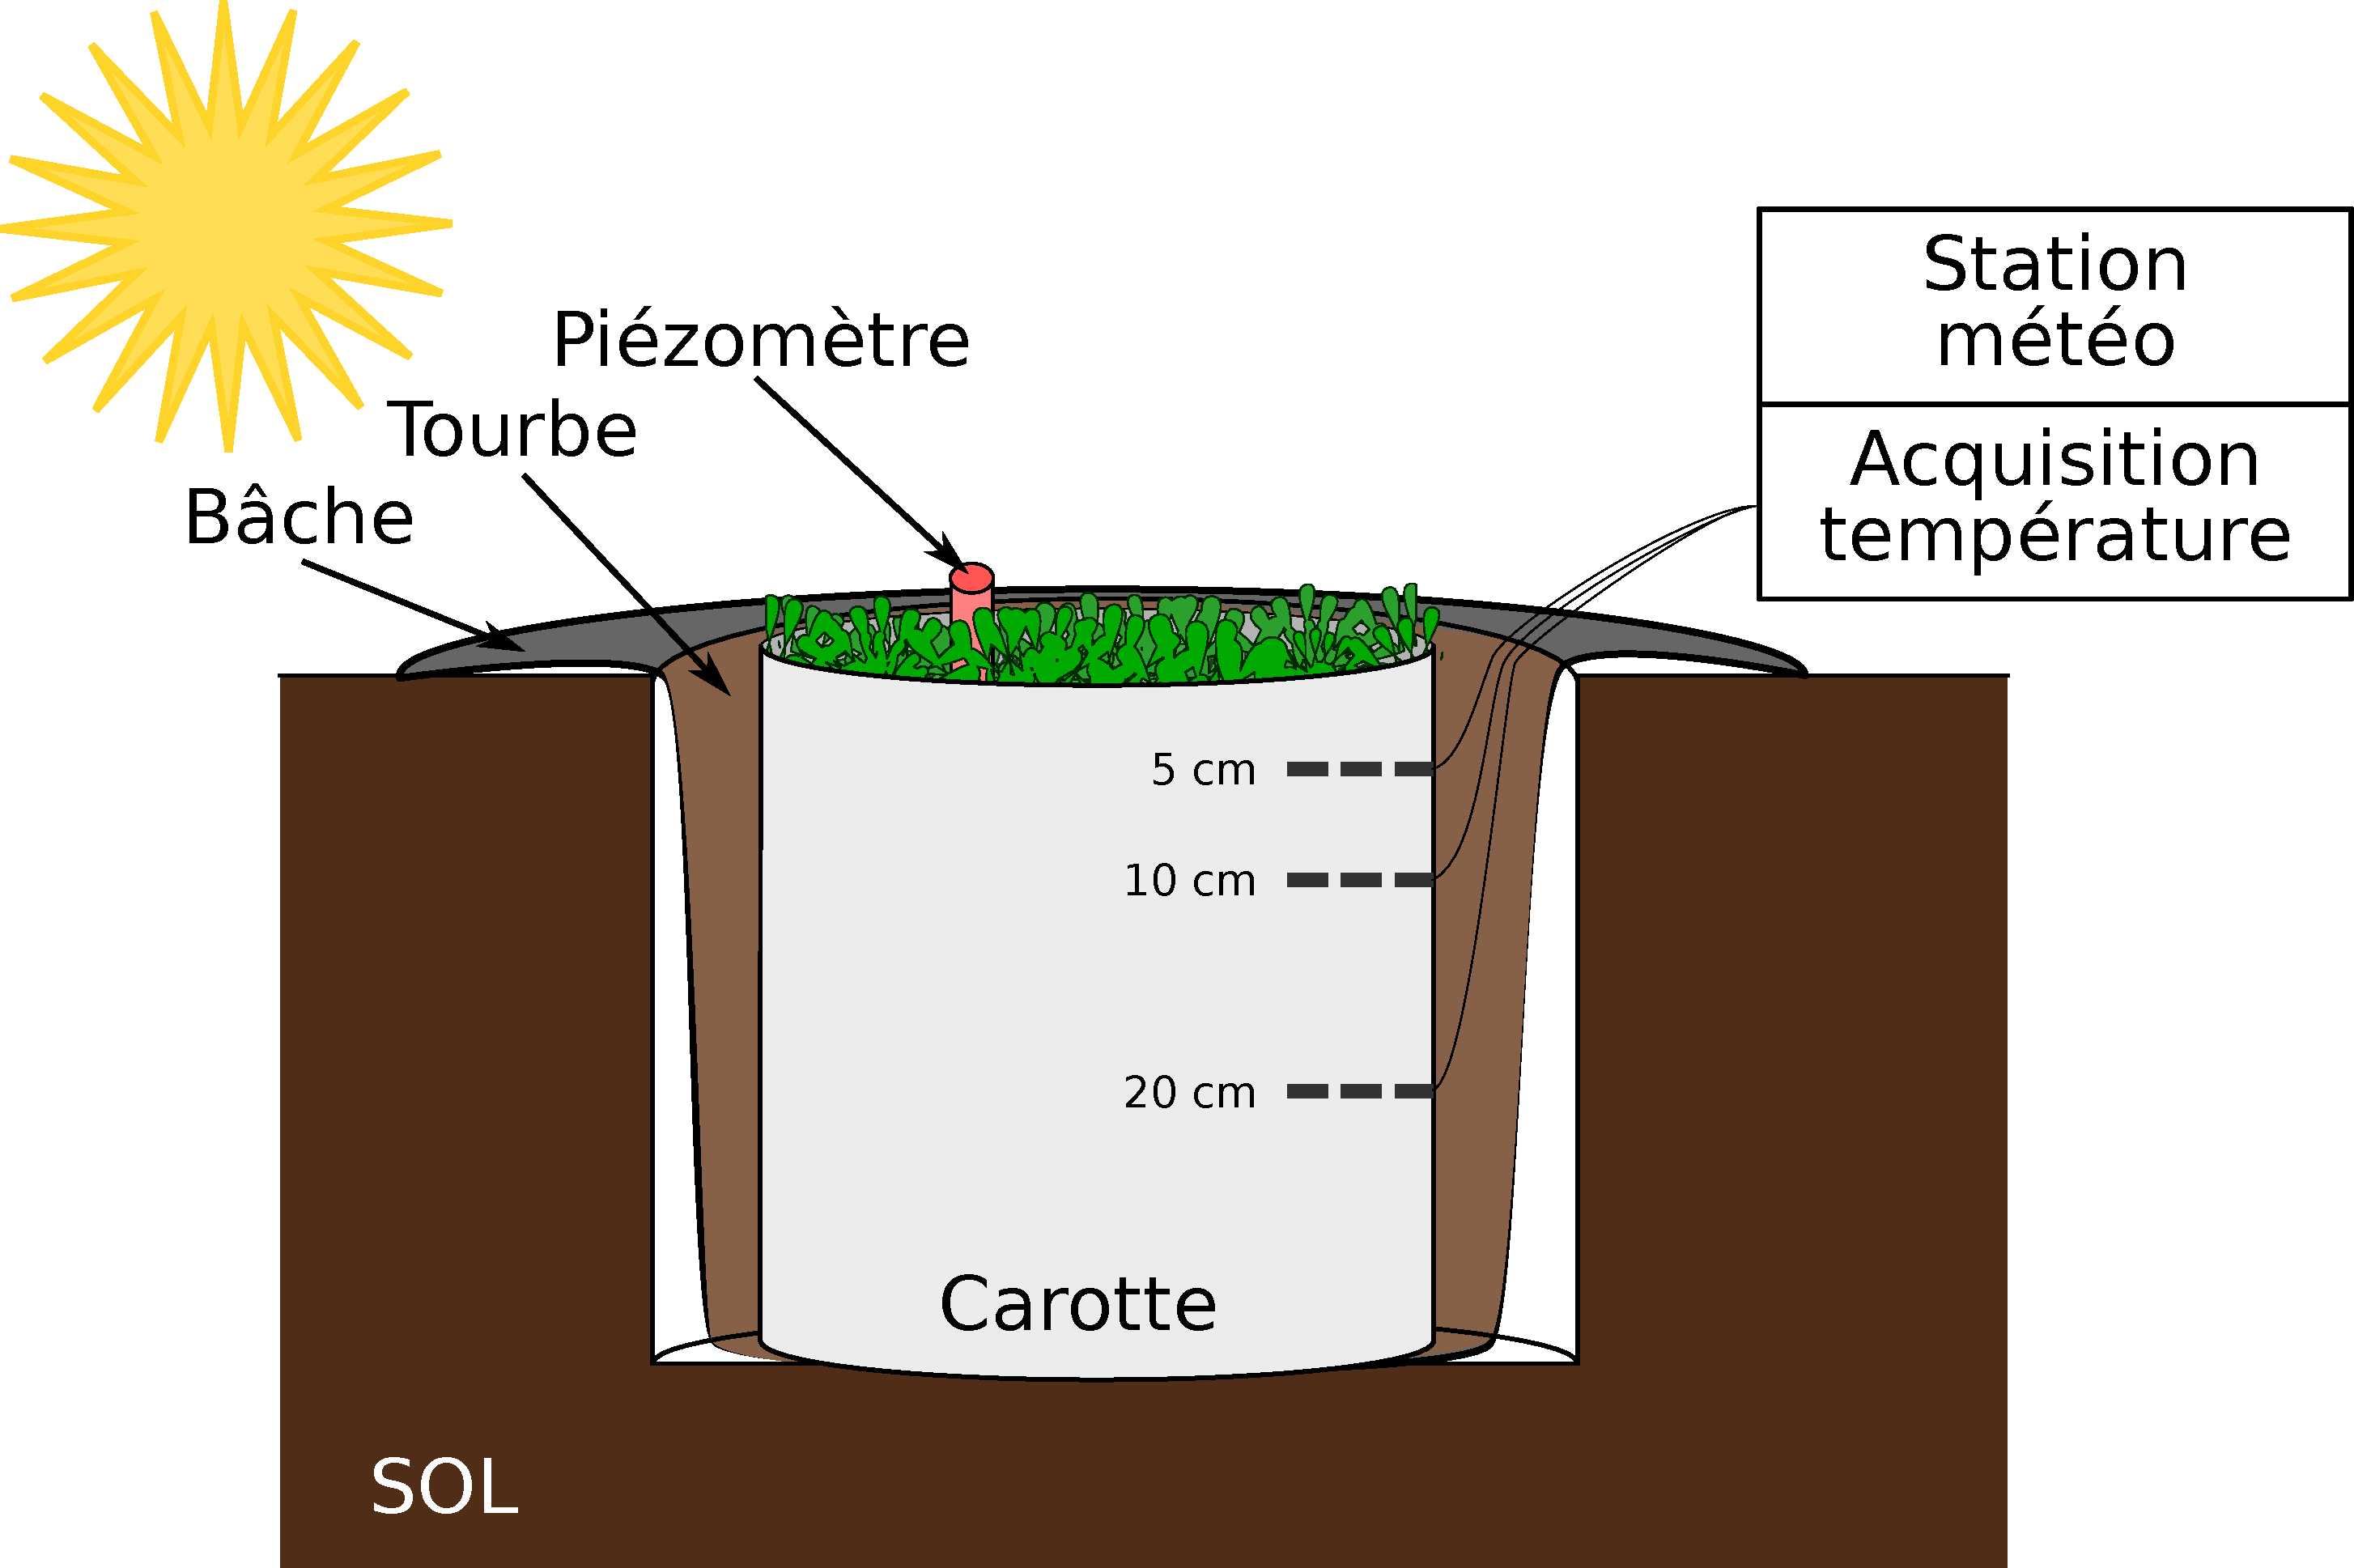
\includegraphics[width=.6\textwidth]{chap4/installation}
%\caption{Dispositif expérimental : les mésocosmes sont installés dans un trou creusé dans le sol. Ils sont isolés de ce dernier par une bâche imperméable et, pour l'expérimentation II, des sondes de température reliées à une station météorologique sont installées à différentes profondeurs.}
%\label{fig:mesocarte}
%\end{figure}


\begin{table}
\centering
\caption{Récapitulatif des différentes phases de dessiccation/réhumectation pour les deux expérimentations. La colonne code phase correspond à la première lettre de la phase (D pour dessiccation et R pour réhumectation) suivi d'un numéro représentant l'ordre du cycle. La phase EQ correspond au temps laissé aux mésocosmes pour s'équilibrer avec leur nouvel environnement.}
\label{table:recap_DR}
\begin{tabular}{llll}\toprule
 & Code phase & Dates & Campagnes \\ \midrule
\multicolumn{4}{l}{Expérimentation I (2013)} \\
 & EQ & 12 avril -- 31 mai & 1 \\ [+.5ex]
 & D1 & 1 juin -- 16 juillet & 2 à 15 \\
 & R1 & 17 -- 20 juillet & 16 à 19 \\
 & D2 & 21 -- 9 août & 20 à 24 \\ [+1ex]
\multicolumn{4}{l}{Expérimentation II (2014)} \\
 & EQ & 17 avril -- 29 juin & 1 à 3 \\ [+.5ex]
 & D1 & 30 juin -- 6 juillet & 4 à 5 \\
 & R1 & 7 -- 16 juillet & 6 à 10 \\ [+.5ex]
 & D2 & 17 -- 28 juillet & 11 à 14\\
 & R2 & 29 juillet -- 3 août & 15 à 17\\[+.5ex]
 & D3 & 4 -- 11 août & 18 à 19\\
 & R3 & 12 -- 14 août & 20 à 21\\
\bottomrule
\end{tabular}
\end{table}


L'étude des cycles de dessiccation/réhumectation est effectuée sur des mésocosmes cylindriques (\SI{30}{\centi\metre} de diamètre et de profondeur), prélevés dans la tourbière de La Guette et installés en extérieur, dans des trous creusés dans le sol.
Au contraire d'échantillons en chambre climatique, cette méthode a l'inconvénient de ne pas permettre un contrôle total des variables expérimentales comme les apports d'eau ou la température.
Cependant, elle permet de maintenir les échantillons dans des conditions plus proches de celles présentes in-situ et notamment le rayonnement solaire, dont la luminosité est inatteignable en chambre climatique.
Deux expérimentations ont été réalisées, la première (expérimentation I) durant l'été 2013 avec un seul cycle long.
Cette expérimentation a été effectuée dans le cadre des stages de Master de Zi Yin de l'Université de Fudan en Chine, qui s'est occupée d'une grande partie de l'acquisition de données de \coo et des facteurs contrôlant et de Paul Gaudry de l'Université d'Orléans qui s'est occupé de faire les mesures de \chh.
%ici à remercier Zi Yin stagiaire de l'Université de Fudan en Chine, qui s'est occupée d'une grande partie de l'acquisition de données de \coo et des facteurs contrôlant et Paul Gaudry stagiaire de l'Université d'Orléans qui s'est occupé de faire les mesures de \chh}.
La seconde (expérimentation II) a été réalisée pendant l'été 2014 avec trois cycles, plus courts et a été effectuée dans le cadre des stages de Master de Tianyi Ji, de l'Université de Fudan en Chine qui s'est occupé de l'acquisition des données \coo, et de Sarah Williams qui a réalisé les mesures de \chh. 

Pour les deux expérimentations, les flux de \coo et de \chh ont donc été suivis ainsi que la température de l'air, du sol (à \SI{-5}{\centi\metre}), le niveau de nappe d'eau, et la teneur en eau du sol pendant les différentes phases de dessiccation et de réhumectation. 

\begin{center}
\begin{minipage}{.85\textwidth}
\setlength{\parindent}{-10pt}%
%\singlespacing
\onehalfspacing
\textbf{Remarque :} % La mesure de la teneur en eau du sol se fait à l'aide d'une sonde munie d'un corps duquel dépasse deux tiges d'une dizaine de centimètre et écartée de deux. 
Pour l'expérimentation I les mesures ont été faites en insérant verticalement la sonde d'une dizaine de centimètres dans le mésocosme.
La mesure est donc une intégration de la teneur en eau sur \SI{10}{\centi\metre}.
En revanche pour l'expérimentation II, la sonde a été insérée horizontalement sur un côté des mésocosmes à une profondeur fixe (\num{-5}, \num{-10} et \SI{-20}{\centi\metre}).
La mesure qui en résulte est donc plus spécifique à cette profondeur.
Pour les deux expérimentations les valeurs obtenues, ne sont pas à prendre de façon absolue, les sondes n'ayant pas été calibrées pour des sols tourbeux mais pour des sols minéraux.
\end{minipage}
\end{center}
%La végétation a été suivie lors de l'expérimentation II.
Les placettes subissant les cycles de dessiccation seront nommées groupe « Dessiccation » et les placettes ne subissant pas les cycles, groupe « Contrôle ».
%Ces deux groupes correspondent aux deux traitements utilisés pour l'analyse statistique.
Pour le \coo et le \chh, l'analyse a été faite sur les flux moyennés sur une journée, les flux ayant été généralement mesurés deux fois par jour.
%Pour le \chh, les flux bruts ont été utilisés.



\subsection{Expérimentation I}
Six mésocosmes ont été prélevés le 12 avril 2013, dans la tourbière de La Guette.
%Le prélèvement s'effectue à l'aide de cylindres de PVC qui, dans un premier temps, posé sur le sol, permettent de faire un pré-découpage au couteau, puis dans un second temps sont insérés, délicatement, dans la tourbe. 
%Les mésocosmes sont finalement dégagés en creusant de chaque côté (Figure~\ref{fig:mesophoto}).
Le prélèvement s'effectue à l'aide de cylindres de PVC, enfoncés délicatement dans la tourbe puis dégagés en creusant de chaque côté (Figure~\ref{fig:mesophoto}).
Enfin ils sont transportés au laboratoire où ils sont installés en extérieur et saturés en eau (eau prélevée dans la tourbière), afin que leurs conditions hydrologiques de départ soient les plus proches possibles.
Trois mésocosmes tirés au sort servent de contrôle, et trois vont subir un cycle de dessiccation/réhumectation.
%À partir du 31 mars 2013 de l'eau a été pompé régulièrement dans les 3 mésocosmes traités pour simuler une sécheresse, jusqu'au 17 juillet.
Du 2 mai au 17 juillet 2013, les précipitations ont été interceptées dans trois mésocosmes à l'aide d'abris bâchés installés en cas de pluie et la nuit (Figure~\ref{fig:mesophoto}).
%À partir du 2 mai 2013 les précipitations ont été interceptées à l'aide d'abri bâchés installés en cas de pluie et la nuit.
%Ces interceptions ont été faites jusqu'au 17 juillet dans les 3 mésocosmes traités pour simuler une sécheresse.
Au 17 juillet, de fortes précipitations sont simulées par l'ajout d'eau de pluie reconstituée\footnote{Cette eau est une eau créée artificiellement, à partir d'un mélange l'eau dé-ionisée, de sulfate de sodium, de nitrate d'ammonium, de chlorures de potassium, de calcium, de magnésium et de sodium pour reproduire la composition d'une eau de pluie.} dans les six mésocosmes (Tableau~\ref{table:recap_DR}).
%À cette date de l'eau est ajouté aux mésocosmes, que ce soit les contrôles ou les traitements, pour simuler de fortes précipitations (Tableau~\ref{table:recap_DR}).
La réhumectation s'est étalée sur quatre jours à raison d'un ajout de \SI{1.16}{\litre} d'eau par jour et par mésocosme reproduisant ainsi un événement pluvieux enregistré dans la tourbière de La Guette (\SI{81.8}{\milli\metre} sur cinq jours).

\subsection{Expérimentation II}
Le 17 avril 2014, six nouveaux mésocosmes ont été prélevés dans la tourbières de La Guette et installés près du laboratoire, en suivant le même protocole que pour l'expérimentation I.
Une station météo a été installée à côté des mésocosmes afin de mesurer avec un pas de 15 minutes la température de l'air, l'humidité relative, le rayonnement solaire, la vitesse et la direction du vent et les précipitations.
La pluviosité n'a pu être enregistrée à cause d'une panne du pluviomètre.
Cette station a permis également l'enregistrement des températures mesurées par les sondes T107 installées à \num{-5}, \num{-10}, et \SI{-20}{\centi\metre}.
Un abaissement manuel du niveau de la nappe a été mis en place pour cette expérimentation, dans le but de pouvoir suivre plusieurs cycles de dessiccation/réhumectation.
%Les conditions météorologiques moins ensoleillée qu'en 2013 et l'objectif de suivre plusieurs cycles de dessiccation/réhumectation ont nécessité la mise en place d'un abaissement manuel du niveau de la nappe.
Pendant les phases d'assèchement les niveaux de nappes des placettes traitées étaient donc abaissés en moyenne de \SI{2}{\centi\metre} par jour, une intensité permettant de simuler plusieurs cycles.
La durée des différents cycles est présentée dans le tableau~\ref{table:recap_DR}.
Pendant les phases de réhumectation, de l'eau de pluie collectée à proximité des mésocosmes, est versée dans les mésocosmes jusqu'à ce que le niveau d'eau atteigne la limite haute de l'embase. 

%Le premier cycle de dessiccation/réhumectation dura du 30 juin au 6 juillet pour la phase de dessiccation est du 7 au 16 juillet pour la phase de réhumectation.
%Le deuxième cycle dura du 17 au 28 juillet et du 29 juillet au 3 aout, 
%Enfin le dernier cycle fut mesuré du 4 au 11 aout pour la dessiccation et du 12 au 14 aout pour la réhumectation (Tableau~\ref{table:recap_DR}).





%\subsection{Analyse des données}



%\begin{table}
%\centering
%\caption{Récapitulatif des mesures pour les deux expérimentations}
%\label{table:recap_hm}
%\begin{tabular}{lll}\toprule
%expérimentation & A & B \\ \midrule
%année & 2013 & 2014 \\
%réplicats & 6 & 6 \\
%cycles & 1 & 3 \\
%station météo & non & oui\\
%\bottomrule
%\end{tabular}
%\end{table}



\section{Résultats}

\subsection{Expérimentation I}

\subsubsection{Dynamique hydrologique}
%\textbf{Dynamique hydrologique}


Pendant la phase de dessiccation on observe une baisse du niveau de la nappe dans les placettes contrôles et dans les placettes traitements (Figure~\ref{fig:HMzi}--A, campagnes 2 à 15).
Cependant si les placettes du groupe « Dessiccation » ont un niveau de nappe qui diminue de façon régulière sur l'ensemble de cette phase, de \num{-3} à \SI{-25}{\centi\metre} ce n'est pas le cas des placettes du groupe « Contrôle ».
Ces dernières ont un niveau de la nappe d'eau qui reste à peu près constant ($\approx$ \SI{-3}{\centi\metre}) entre les campagnes 4 et 8, du fait d'épisodes pluvieux pendant cette période.
Puis le niveau de nappe diminue entre les campagnes 9 et 15, passant de \num{-7} à \SI{-22}{\centi\metre}.
%Le niveau de nappe d'eau dans le groupe « Dessiccation » passe de \num{-3} à \SI{-25}{\centi\metre} pendant cette phase.
Pendant la phase de réhumectation, les deux groupes ont un comportement similaire.
Leurs niveaux de nappe augmentent de \num{-22} à \SI{-1}{\centi\metre} pour le groupe « Contrôle » et de \num{-25} à \SI{-1}{\centi\metre} pour le groupe « Dessiccation ».
Dans la seconde phase d'assèchement le niveau de nappe baisse à nouveau pour les deux groupes, de façon régulière pour le groupe « Dessiccation » jusqu'à atteindre une profondeur de \SI{-30}{\centi\metre}, et de façon plus irrégulière à cause des pluies, pour le groupe « Contrôle ».

%Dans le même temps le niveau de nappe du groupe « Dessiccation » diminue (\num{-10} à \SI{-15}{\centi\metre})
%Entre les campagnes 9 à 15 le niveau de nappe diminue pour les deux groupes.
%De \num{-7} à \num{-22} et de \num{-18} à \SI{-25}{\centi\metre} respectivement pour les groupes « Contrôle » et « Dessiccation ».
%La réhumectation commence par une augmentation du niveau de la nappe importante des campagnes 15 à 18 : il passe de \num{-22} à \SI{-4}{\centi\metre} pour le groupe « Contrôle » et de \num{-25} à \SI{-5}{\centi\metre} pour le groupe « Dessiccation ».
%Dans une seconde phase de la réhumectation, des campagnes 18 à 20, le niveau de nappe n'évolue plus que faiblement, oscillant entre -5 et \SI{-1}{\centi\metre} pour les deux groupes. 

Cette dynamique d'assèchement est également visible à travers l'évolution de la teneur en eau du sol (Figure~\ref{fig:HMzi_T}--A).
Pour le groupe « Contrôle », la teneur en eau se maintient à \SI{100}{\percent} jusqu'à la campagne 5 puis elle diminue jusqu'à la campagne 15 où elle atteint \SI{43}{\percent}.
La teneur en eau du sol du groupe « Dessiccation » diminue dès la campagne 2 et atteint \SI{41}{\percent} à la fin de la phase de dessiccation (campagne 15).
À ce moment les deux groupes sont relativement proches.
Ils le restent lors de la phase de réhumectation pendant laquelle la teneur en eau du sol augmente.
Cette dernière augmente même pendant la 2\ieme phase de dessiccation, jusqu'à la campagne 22 pour le groupe « Contrôle » et 20 pour le groupe « Dessiccation », où elle atteint 100 et \SI{86}{\percent} respectivement.

%Cette dynamique d'assèchement s'observe également au niveau de la teneur en eau du sol (Figure~\ref{fig:expA_SWC_T}).
%Des campagnes 4 à 8 la teneur en eau du sol diminue de 100 à \SI{64}{\percent}.
%Dans le même temps la teneur en eau du sol (87 à \SI{53}{\percent}).
%Entre les campagnes 9 à 15  les groupes « Contrôle » et « Dessiccation » se retrouve également proche en termes de teneur en eau du sol : 41 et \SI{43}{\percent} respectivement.
%Campagnes 15 à 18  la teneur en eau du sol varie peu, de 43 à 57 et de 41 à \SI{56}{\percent} respectivement pour les groupes « Contrôle » et « Dessiccation ».
%Dans une seconde phase de la réhumectation, des campagnes 18 à 20, la teneur en eau du sol continue d'augmenter passant de 57 à \SI{90}{\percent} pour le groupe « Contrôle » et de 56 à \SI{86}{\percent} pour le groupe « Dessiccation »

La réponse hydrologique au cycle de dessiccation/réhumectation est différente selon qu'on l'observe à travers le niveau de la nappe ou la teneur en eau du sol (Figure~\ref{fig:wtlSWC_A}).
Pendant la dessiccation du groupe « Contrôle » le niveau de nappe reste, dans un premier temps, constant jusqu'à la campagne n°8 puis il diminue. 
Pendant la phase de réhumectation, ce même groupe suit un « chemin » identique, le niveau de nappe commence par augmenter avec une variation limitée de la teneur en eau du sol jusqu'à la campagne n°18, puis par la suite, la teneur en eau du sol augmente tandis que le niveau de nappe reste plus constant voire diminue.
Pour le groupe « Dessiccation », on observe une diminution conjointe du niveau de nappe et de la teneur en eau lors de la phase de dessiccation.
Cette relation n'est cependant pas strictement linéaire avec une teneur en eau qui varie peu pendant les trois premières campagnes, puis qui diminue jusqu'à la campagne n°8, avant de diminuer de manière moins importante jusqu'à la fin de la phase de dessiccation.
Le niveau de nappe du groupe « Dessiccation » diminue de façon régulière pendant cette phase.
À l'inverse du groupe « Contrôle » la phase de réhumectation du le groupe « Dessiccation », ne suit pas le même chemin que lors de la dessiccation.
Pendant la réhumectation le chemin est très proche de celui observé pour le groupe « Contrôle » avec un niveau de nappe qui commence par augmenter, avant de se stabiliser et, pendant cette stabilisation, une augmentation de la teneur en eau du sol.
Au delà de la campagne n°20 le comportement des groupes diverge à nouveau.
Le groupe « Contrôle » semble reprendre le même chemin de dessiccation à l'exception d'un point.
Ce point, (campagne n°23) et liée à une baisse brusque du niveau de la nappe (\SI{-18}{\centi\metre}) et semble davantage sur le « chemin » du groupe « Dessiccation ».
Le groupe dessiccation quant à lui suit un chemin proche de sa première phase de dessiccation même si la teneur en eau du sol diminue moins rapidement par rapport au niveau de la nappe que précédemment.


\begin{figure}
\centering
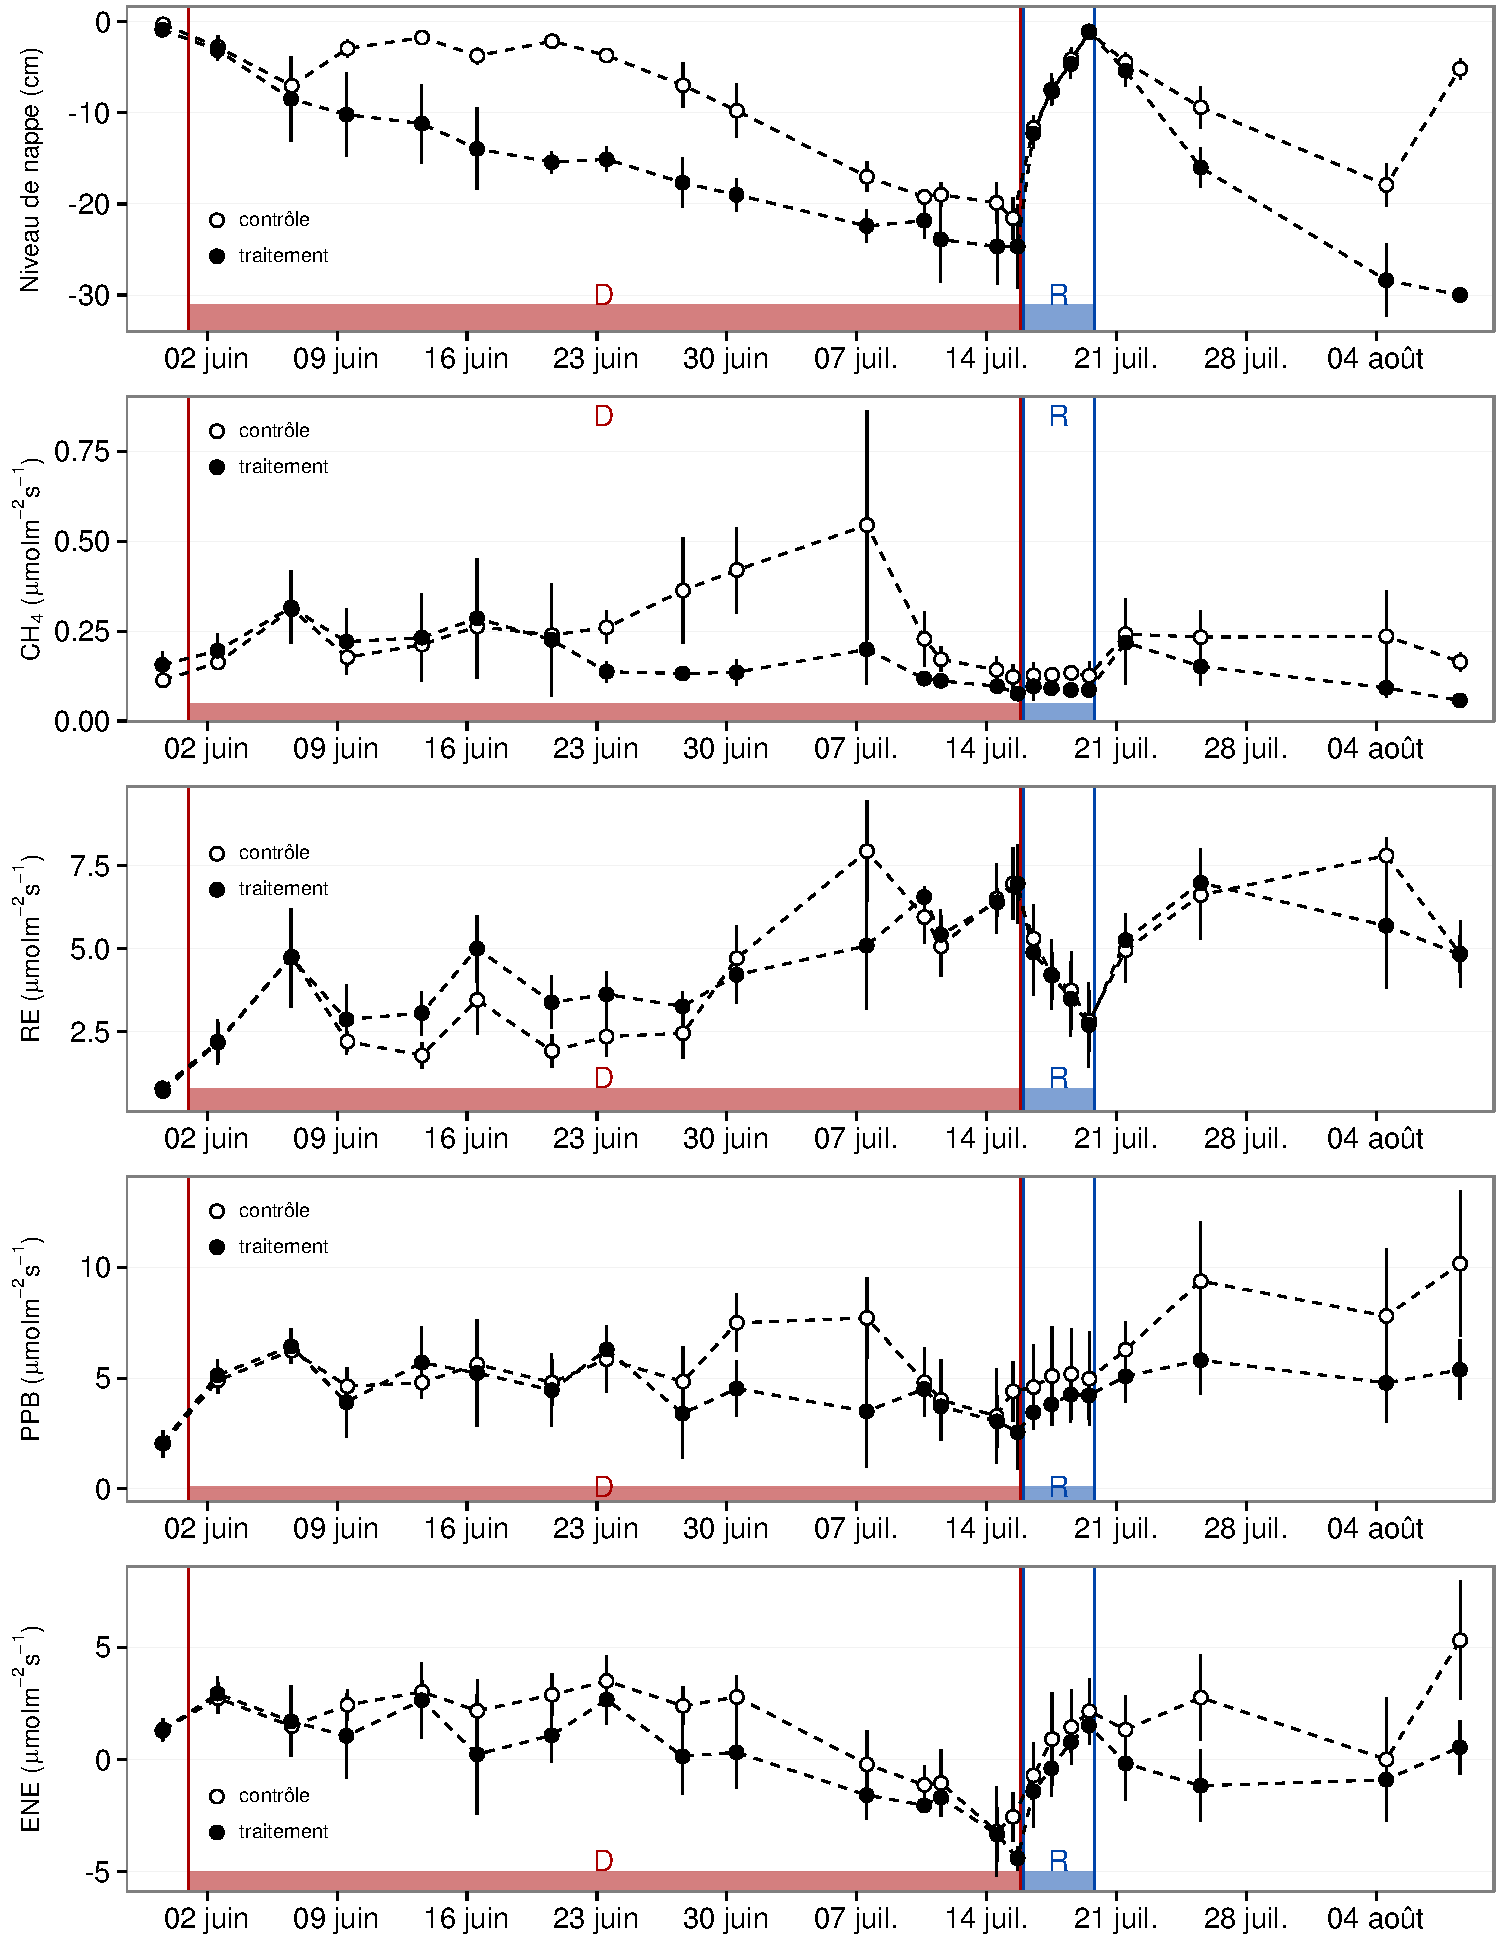
\includegraphics[width=1.15\textwidth, center]{chap4/expA_flux}
\caption{Expérimentation I : Évolution de la moyenne journalière du niveau de nappe en cm (A), et des flux, \chh, RE, PPB, ENE en \si{\uml}, B, C, D, E de juin à août 2013, dans les placettes « Contrôle » et « Dessiccation ». Les phases de dessiccation (D) sont représentées en rouge et la phase de réhumectation (R), en bleu. Les numéros de 1 à 24 correspondent aux dates des campagnes.}
\label{fig:HMzi}
\end{figure}

\begin{figure}
\centering
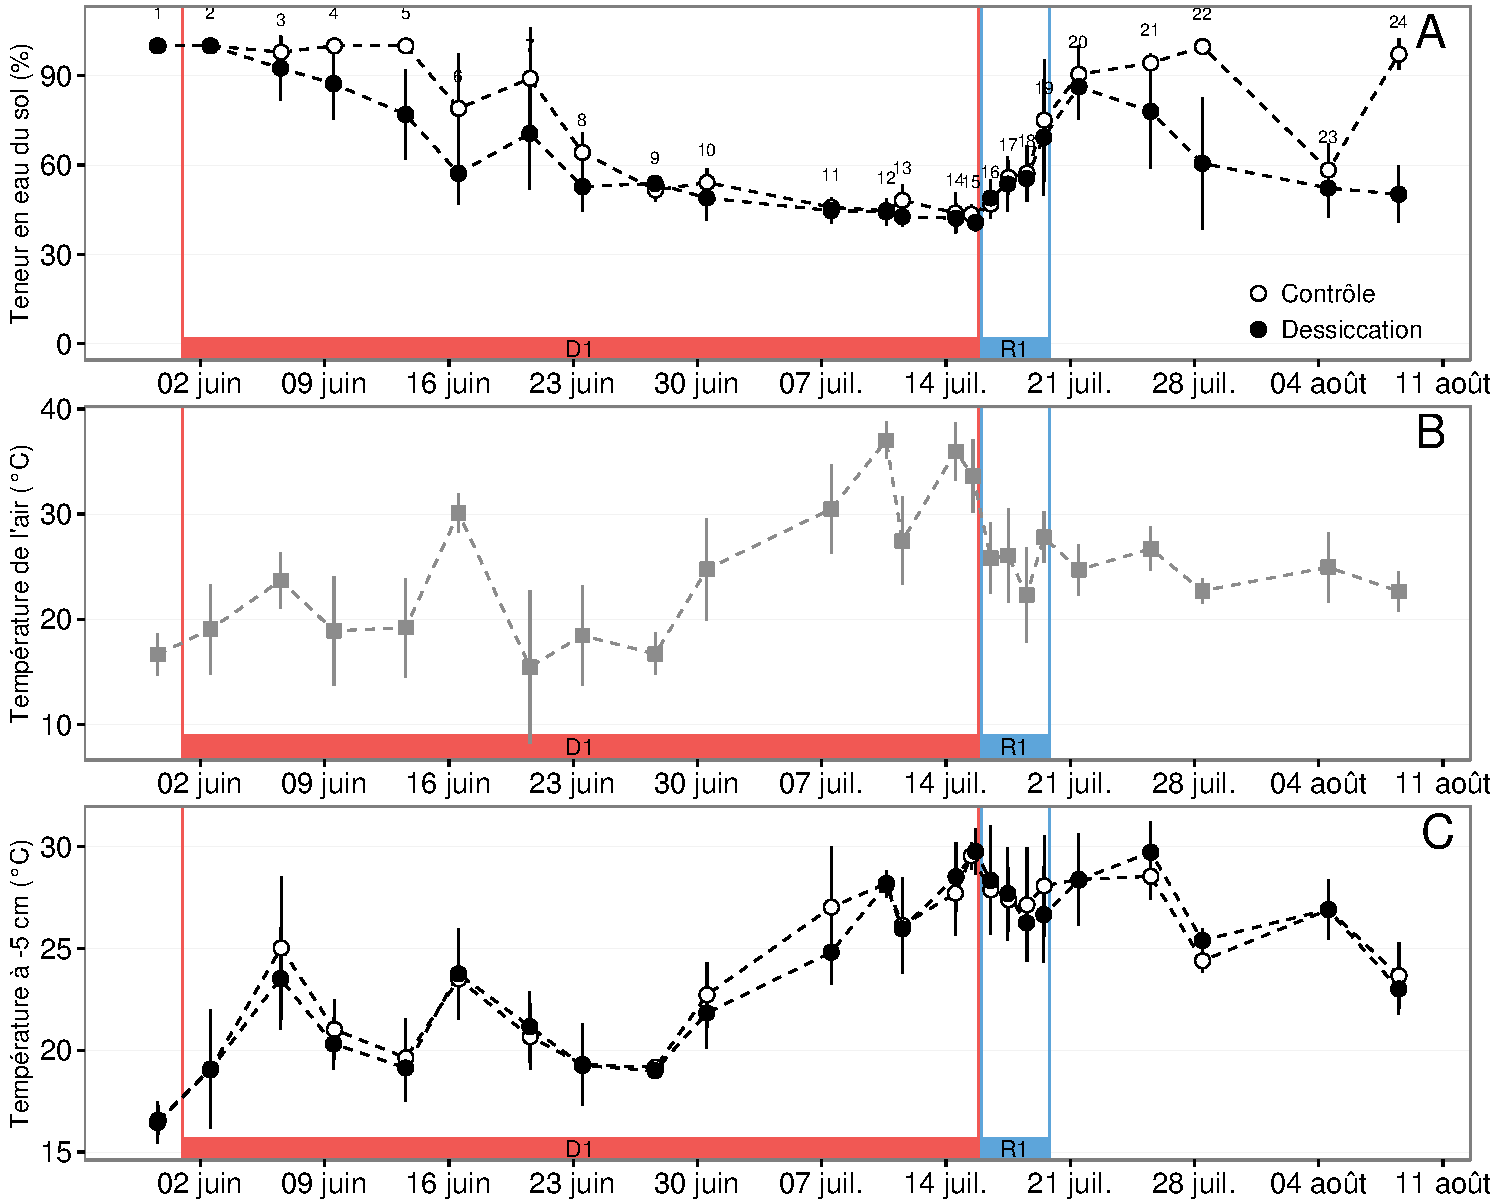
\includegraphics[width=1.15\textwidth, center]{chap4/expA_SWC_T}
\caption{Expérimentation II : Évolution de la teneur en eau du sol à \SI{-5}{\centi\metre} (A), de la température de l'air (B), et de la température du sol à \SI{-5}{\centi\metre} (C) de juin à août 2013, dans les placettes « Contrôle » et « Dessiccation ». Les phases de dessiccation (D) sont représentées en rouge et la phase de réhumectation (R), en bleu. Les numéros de 1 à 24 correspondent aux dates des campagnes.}
\label{fig:HMzi_T}
\end{figure}


\begin{figure}
\centering
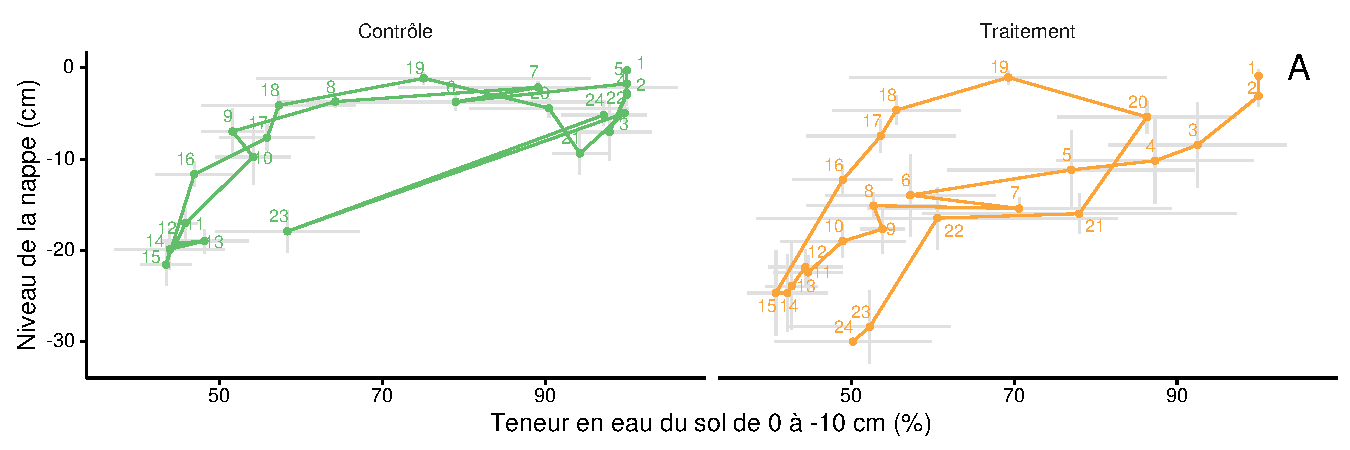
\includegraphics[width=1.15\textwidth, center]{chap4/expA_wtlSWC}
\caption{Relation entre les niveaux de nappe et la teneur en eau du sol lors de l'expérimentation I. Les numéros correspondent à l'ordre des campagnes de mesures et les lignes grises aux déviations standards.}
\label{fig:wtlSWC_A}
\end{figure}

\subsubsection{Les flux de \chh}

Les émissions de \chh varient dans l'ensemble de 0 et \SI{0.55}{\uml}.
Elles sont similaires entre les deux groupes (« Contrôle » et « Dessiccation ») jusqu'à la campagne n°8 à partir de laquelle elles divergent (Figure~\ref{fig:HMzi}--B).
À partir de cette campagne, les émissions du groupe « Contrôle » augmentent rapidement pour atteindre \SI{0.55(031)}{\uml} tandis que celles du groupe « Dessiccation » restent stables, voire diminue légèrement.
À la fin de la phase de dessiccation, mi-juillet, les deux groupes retrouvent des niveaux d'émission similaires compris entre \num{0.1} et \SI{0.2}{\uml}.
Ces niveaux restent constants pendant toute la phase de réhumectation, avant d'augmenter légèrement pendant la deuxième phase de dessiccation pour se situer entre \SI{0.25}{\uml} et \SI{0.2}{\uml}.

\subsubsection{La RE}

Pendant la phase de dessiccation, les flux de la RE tendent à augmenter quel que soit le groupe de placettes considéré (Figure~\ref{fig:HMzi}--C).
Ces valeurs inférieures à \SI{2.5}{\uml} début juin, atteignent environ \SI{7}{\uml} pour les deux groupes mi-juillet, avant la réhumectation.
La RE du groupe « Dessiccation » est supérieure à celle du groupe « Contrôle » pendant une grande partie du mois de juin.
Cependant la RE du groupe « Dessiccation » augmente régulièrement pendant l'ensemble de cette phase jusqu'à \SI{3.26(046)}{\uml}, tandis que les valeurs du groupe « Contrôle » restent, dans un premier temps, stables jusque fin juin (\SI{2.45(075)}{\uml}).
%La RE de ce groupe vaut alors \SI{2.45(075)}{\uml} contre \SI{3.26(046)}{\uml} pour le groupe traité.
%Cet écart, pouvant varier dans le temps,  étant installé depuis le 9 juin
À partir de début juillet, les valeurs de RE du groupe « Contrôle » augmentent jusqu'à dépasser les valeurs du groupe « Dessiccation ».
La Re de ce groupe atteint un maximum à \SI{7.93(152)}{\uml} le 8 juillet avant de retrouver des valeurs proches de celles observées dans le groupe « Dessiccation ».
Cette augmentation brusque correspond temporellement à celle observée, pour le même groupe, dans les flux de \chh.
Lors de la phase de réhumectation, les flux de RE diminuent de façon très similaire pour les deux groupes pour atteindre \SI{2.75}{\uml} lors de la campagne n°19.
Ce minimum reste cependant plus élevé que les valeurs mesurées initialement (\SI{0.7}{\uml}).
Après la phase de réhumectation, les flux des deux groupes restent relativement proches et augmentent à mesure que le niveau de la nappe diminue à nouveau (Figure~\ref{fig:HMzi}--A).

\subsubsection{La PPB}

Pour les deux groupes, les flux de PPB restent stables pendant la phase de dessiccation (Figure~\ref{fig:HMzi}--D) :
entre 5 et \SI{6}{\uml} (\SI{5.29(076)}{\uml} de moyenne pour les deux groupes) jusqu'au 24 juin.
Ensuite, comme pour le \chh et la RE, les valeurs de la PPB du groupe « Contrôle » augmentent et s'écartent de celles mesurées dans le groupe « Dessiccation ».
À la fin de cette phase de dessiccation, les flux redeviennent identiques entre les traitements et atteignent un minimum proche de \SI{3}{\uml}.
Pendant la phase de réhumectation, la PPB augmente légèrement pour les deux groupes.
La PPB dans le groupe de contrôle a des valeurs supérieures à celles du groupe « Dessiccation ».
Pendant la deuxième phase de dessiccation, la PPB augmente pour les deux groupes, avec un maximum de \SI{5.83(161)}{\uml} pour le groupe « Dessiccation » et de \SI{10.17(330)}{\uml} pour le groupe « Contrôle ».

\subsubsection{L'ENE}

%L'ENE est systématiquement supérieure pour le groupe « Contrôle », avec une cinétique parallèle des flux pour les deux groupes
Pour l'ensemble de l'expérimentation, les flux d'ENE varient de la même façon et sont plus élevés dans le groupe « Contrôle » que ceux du groupe « Dessiccation » (Figure~\ref{fig:HMzi}--E).
Pendant la phase de dessiccation, l'ENE reste relativement constante jusque fin juin (campagne n°10) avec une valeur moyenne pour les deux groupes de \SI{1.18(058)}{\uml}.
%L'écart entre le groupe « Contrôle » et le groupe « Dessiccation » tend à augmenter du 10 au 30 juin environ, avant que les valeurs du groupe de « Contrôle » ne rejoignent celles du groupe « Dessiccation ».
Au delà du 30 juin (campagne n°10), l'ENE baisse pour les deux groupes pour atteindre un minimum proche de \SI{-4.5}{\uml} (campagne n°15).
Pendant la phase de réhumectation, l'ENE augmente rapidement pour atteindre \num{1.52(036)} et \SI{2.15(147)}{\uml} pour le groupe « Contrôle » et de groupe « Dessiccation » respectivement (campagne n°19).
Après la réhumectation, l'ENE du groupe « Contrôle » varie en suivant généralement les variations du niveau de nappe.
Pour le groupe « Dessiccation », l'ENE baisse par rapport au maximum atteint lors de la réhumectation puis se stabilise autour de 0.

\subsubsection{Météorologie}

Pendant la première phase de dessiccation (mois de juin), les températures de l'air restent plus ou moins stables autour d'une valeur de \SI{26}{\degreeCelsius} jusqu'à la campagne n°9, puis elles augmentent jusqu'à la fin de la phase de dessiccation où elles atteignent \SI{42}{\degreeCelsius} (Figure~\ref{fig:HMzi}--B).
Les températures de l'air diminuent pendant la réhumectation puis restent stables avec des valeurs proches de \SI{22}{\degreeCelsius}.
Les températures du sol à \SI{-5}{\centi\metre} de profondeur suivent les même tendances que la température de l'air, à l'exception d'une baisse moins prononcée suite à la réhumectation (Figure~\ref{fig:HMzi}--C).


\subsubsection{Synthèse des résultats de l'expérimentation I}


Les variations de la RE sont principalement liées aux variations du niveau de la nappe (Figure~\ref{fig:hm_wtl}--C).
Par conséquent, les variations de RE se répercutent sur l'ENE (Figure~\ref{fig:hm_wtl}--G).
L'effet des variations du niveau de la nappe sur la PPB est quasiment nul (Figure~\ref{fig:hm_wtl}--E), même si la PPB semble diminuer aux plus fortes profondeurs.
Pour le \chh il est difficile de distinguer des tendances générales entre les flux et les niveaux de nappe (Figure~\ref{fig:hm_wtl}--A).

\subsection{Expérimentation II}

Cette expérimentation est basée sur le suivi de trois phases de dessiccation chacune suivie d'une phase de réhumectation.

\subsubsection{Dynamique hydrologique}

\begin{figure}
\centering
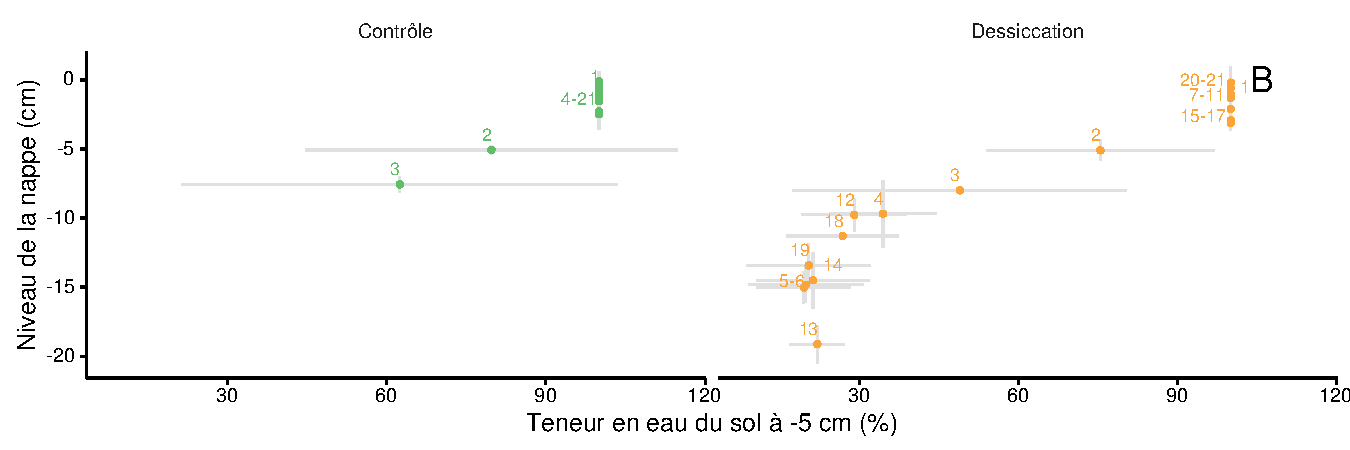
\includegraphics[width=1.15\textwidth, center]{chap4/expB_wtlSWC}
\caption{Relation entre les niveaux de nappe et la teneur en eau du sol lors de l'expérimentation II. Les numéros correspondent à l'ordre des campagnes de mesures et les lignes grises aux déviations standards.}
\label{fig:wtlSWC_B}
\end{figure}

Contrairement à l'expérimentation I, le niveau de nappe du groupe « Contrôle » de l'expérimentation II reste relativement constant pendant l'ensemble de la période de mesures (Figure~\ref{fig:HMty}--A).
Le drainage artificiel du groupe « Dessiccation » conduit à une diminution du niveau de la nappe d'une quinzaine de centimètres en moyenne pour chaque cycle et un temps pluvieux permet au groupe « Contrôle » de garder un niveau de nappe constant et élevé, supérieur à \SI{-5}{\centi\metre} la plupart du temps.
Ce dernier n'a baissé dans les « Contrôle »s », avec la teneur en eau du sol, que lors des campagnes 2 et 3 où il atteint son point le plus bas à \SI{-8}{\centi\metre}.
Les niveaux de nappe minimum des différents cycles sont \num{-15}, \num{-19} et \SI{-13}{\centi\metre} respectivement pour D1, D2 et D3.

La teneur en eau du sol à \SI{-5}{\centi\metre} est constante, à \SI{100}{\percent} pour le groupe contrôle, à l'exception des campagnes n°2 et 3 ou elle baisse et atteint \SI{93}{\percent} (Figure~\ref{fig:HMty_T}--A).
Pour le groupe « Dessiccation », la teneur en eau du sol à \SI{-5}{\centi\metre} est proche de \SI{20}{\percent} pendant les phases de dessiccation et vaut \SI{100}{\percent} pendant les phases de réhumectation.
Les teneurs en eau mesurées à \num{-10} et \SI{-20}{\centi\metre} valent \SI{100}{\percent} pour l'ensemble de l'expérimentation.

Lors de cette expérimentation et compte tenu de la durée de chaque cycle, le nombre de points par cycle est moins important que pour l'expérimentation I.
Il est donc difficile de voir si le comportement et les relations teneur en eau de sol/niveau de nappe varient selon les phases d'un même cycle et entre les cycles (Figure~\ref{fig:wtlSWC_B}).
%De façon générale pour le groupe « Dessiccation », lors des phases de dessiccation les niveaux de nappes sont compris entre \num{-10} et \SI{-20}{\centi\metre} et les teneurs en eau du sol entre 35 et \SI{20}{\percent}.
%Lors des phases de réhumectations les niveaux de nappes sont compris entre \num{0} et \SI{-7}{\centi\metre} et les teneurs en eau du sol restent à \SI{100}{\percent}.

%À l'exception du point mesuré lors de la première phase de dessiccation, les valeurs du groupe de contrôle sont systématiquement supérieures à celles du groupe traité.


\begin{figure}
\centering
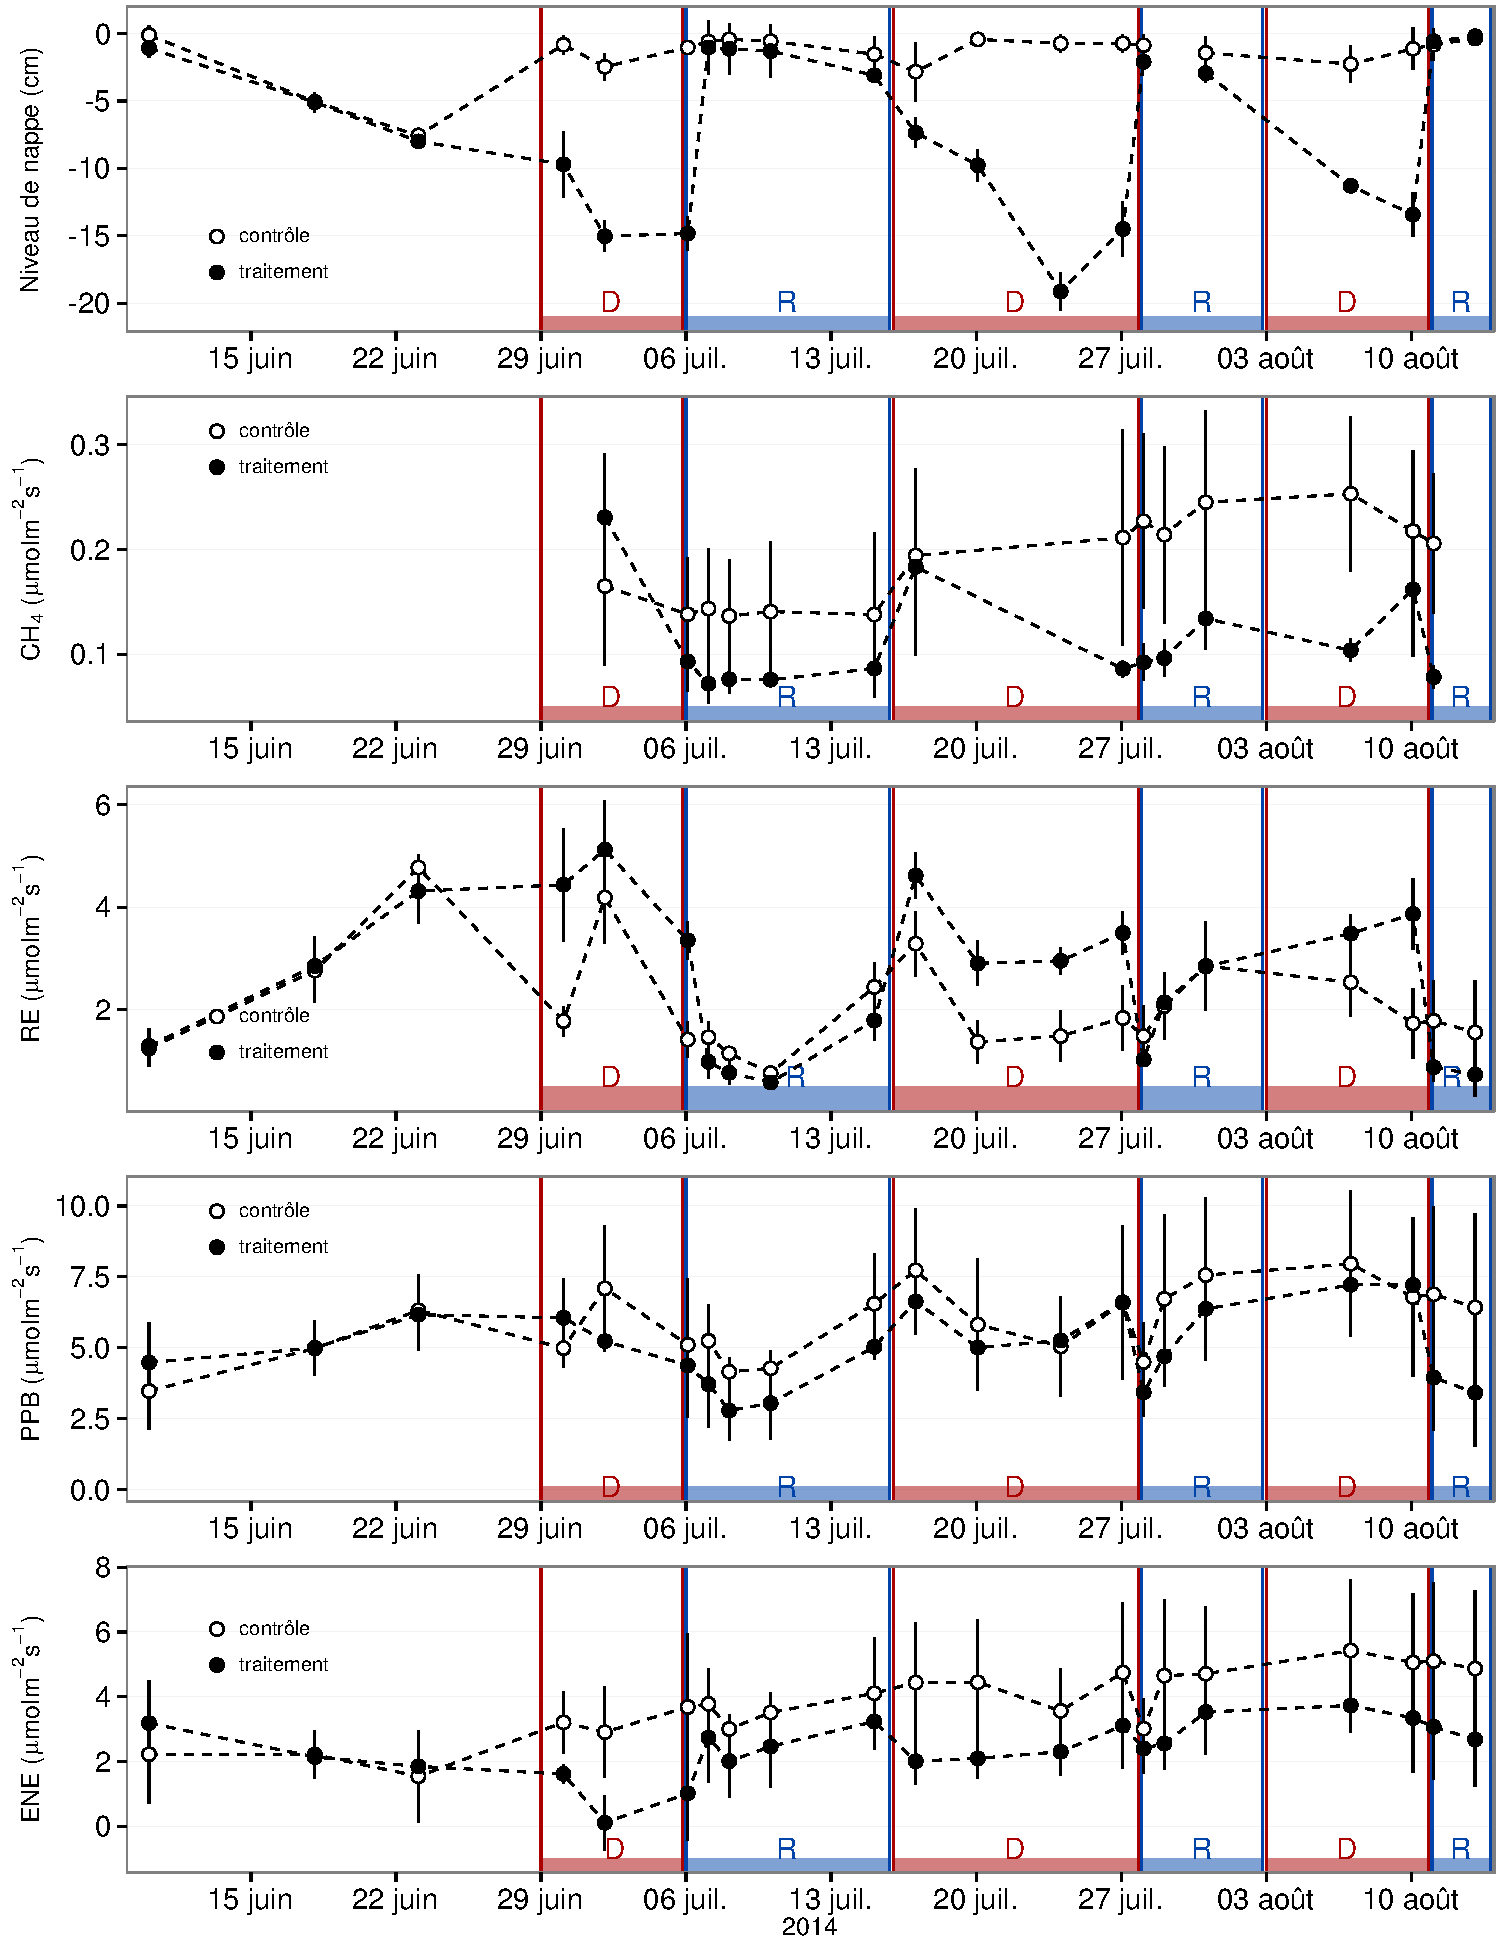
\includegraphics[width=1.15\textwidth, center]{chap4/expB_flux}
\caption{Expérimentation II : Moyenne journalière du niveau de nappe en cm (A), et des flux, \chh, RE, PPB, ENE en \si{\uml}, B, C, D, E. Les cadres et bandes colorées correspondent aux phases de dessiccation (D) en rouge et aux phases de réhumectation (R) en bleu. Les numéros présents sur le graphe A correspondent aux numéros des campagnes.}
\label{fig:HMty}
\end{figure}

\begin{figure}
\centering
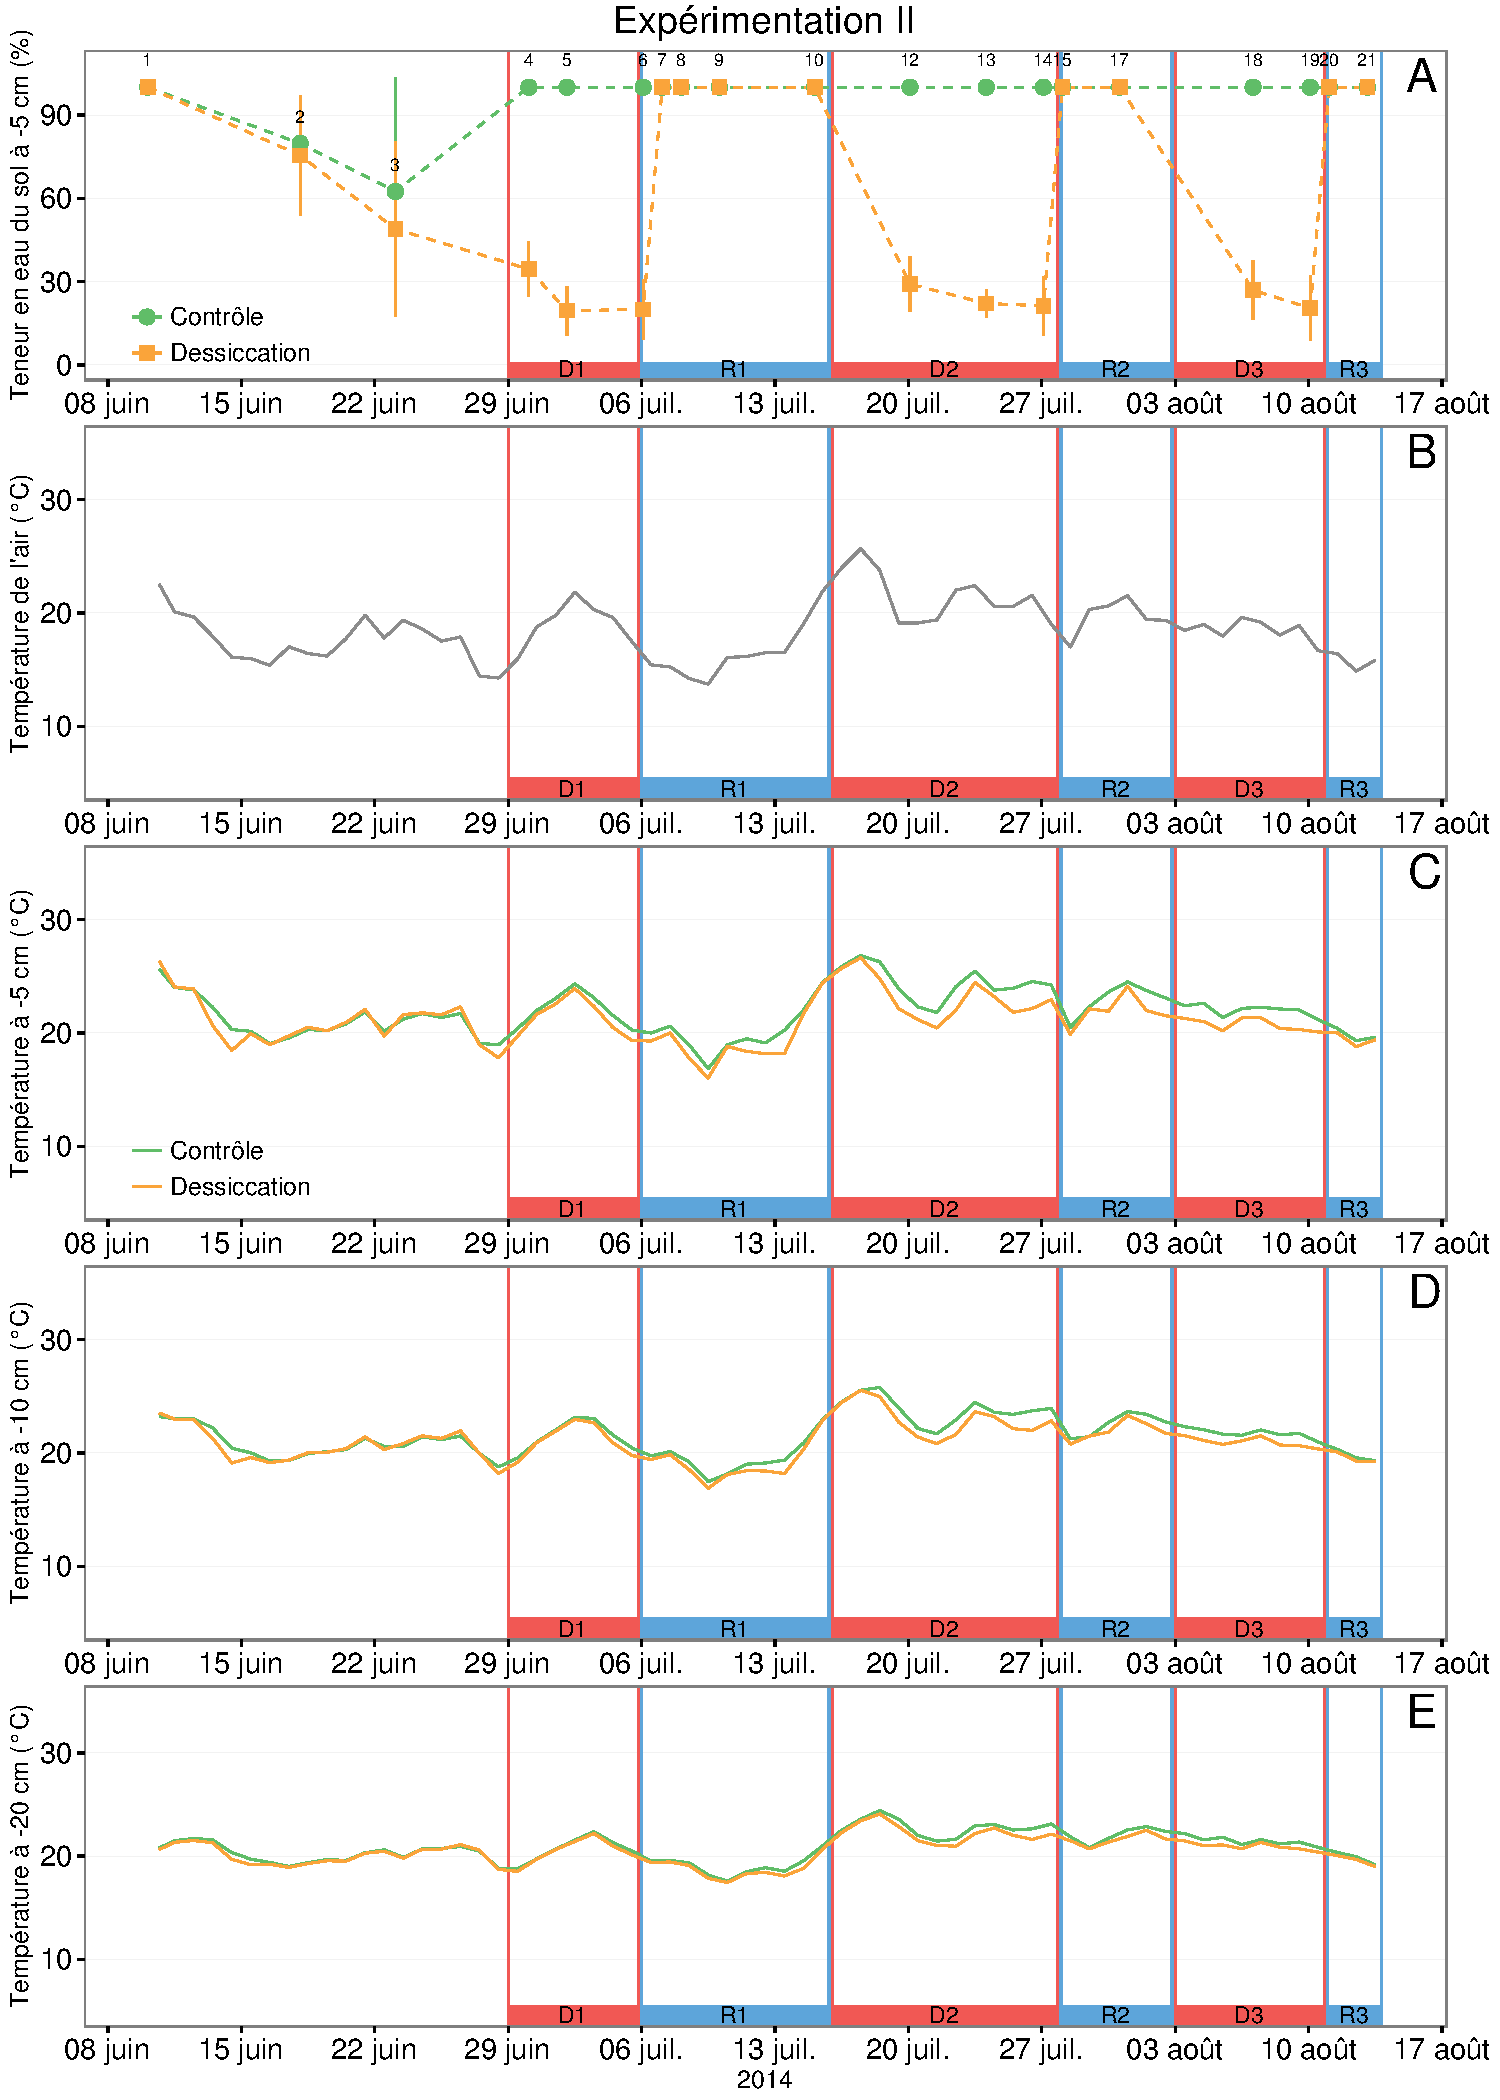
\includegraphics[width=1.15\textwidth, center]{chap4/expB_SWC_T}
\caption{Expérimentation II : Évolution de la teneur en eau du sol à \SI{-5}{\centi\metre} (A), de la température de l'air (B), et des températures du sol à \num{-5}, \num{-10}, \SI{-20}{\centi\metre} (C, D, E). Les cadres et bandes colorées correspondent aux phases de dessiccation (D) en rouge et aux phases de réhumectation (R) en bleu. Les numéros présents sur le graphe A correspondent aux numéros des campagnes.}
\label{fig:HMty_T}
\end{figure}


\subsubsection{Les flux de \chh}

Les flux moyens de \chh varient entre \num{0.07} à \SI{0.34}{\uml} (Figure~\ref{fig:HMty}--B).
Dans l'ensemble, les flux du groupe « Contrôle », à l'exception de la première mesure, sont supérieurs aux flux du groupe « Dessiccation » : moyennes globales de \num{0.20(006)} et \SI{0.11(005)}{\uml}, respectivement).
Les émissions du groupe « Contrôle » tendent à augmenter sur la période de mesure.
Une tendance similaire, est également visible pour le groupe « Dessiccation ».
Concernant les cycles de dessiccation/réhumectation, il est difficile de dégager des comportements communs entre eux.
Le passage de la phase R1 à D2 semble provoquer une émission importante de \chh  (Figure~\ref{fig:HMty}--B).
Cette émission se maintient pour le groupe « Contrôle » et ne dure pas pour le groupe « Dessiccation ».
Pour le goupe « Dessiccation » il semble également y avoir un pic de \chh à la fin de la phase D3.
La relation entre le \chh et le niveau de nappe n'est pas plus visible en rassemblant l'ensemble des données (Figure~\ref{fig:hm_wtl}--B).

\subsubsection{La RE}

La RE varie pour les deux groupes entre \num{0.42} et \SI{5.12}{\uml} (Figure~\ref{fig:HMty}--C)).
Avant le démarrage des manipulations du niveau de la nappe, les valeurs des deux groupes sont très proches et augmentent tandis que le niveau de nappe diminue.
Pendant les phases de dessiccation, les valeurs du groupe « Dessiccation » sont systématiquement supérieures, de \num{1.5} à \SI{1.8}{\uml} en moyenne par phase, par rapport à celles du groupe « Contrôle ».
À l'inverse pendant les phases de réhumectation, les flux entre les deux groupes sont beaucoup plus proches avec une tendance de la RE du groupe « Contrôle » à être supérieure à celle du groupe « Dessiccation ».
La RE du groupe traité est systématiquement plus faible pendant les phases de réhumectation que pendant les phases de dessiccation.
En moyenne la RE vaut respectivement \num{2.28(100)} et \SI{3.86(080)}{\uml} pour les groupes « Contrôle » et « Dessiccation » pendant les phases de dessiccation et \num{1.70(062)} et \SI{1.51(098)}{\uml} pendant les phases de réhumectation.
%Avant le début des traitement d'assèchement, les flux de la RE sont proches pour les deux groupes tandis qu'après, leurs comportements diffèrent (Figure~\ref{fig:HMty}--C)).
%Pendant les phases de dessiccation la RE du groupe traité est supérieure à celle du groupe de contrôle.
%La relation semble s'inverser pendant les phases de réhumectation, du moins pour les cycles 1 et 3, car pendant la phase de réhumectation du cycle 2 les deux groupes ont des valeurs similaires.
\subsubsection{La PPB}

Sur l'ensemble de la période de mesure, la PPB est comprise entre \num{2.78} et \SI{7.96}{\uml} (Figure~\ref{fig:HMty}--D).
Avant le début des traitements, les flux des deux groupes sont similaires.
À partir de la première phase de dessiccation, la PPB du groupe « Contrôle » est supérieure à celle du groupe « Dessiccation ».
Pour les deux groupes, la PPB est plus importante lors des phases de dessiccation comparée aux phase de réhumectation, avec des moyennes respectives de \num{6.35(219)} contre \num{5.80(220)} pour le groupe « Contrôle » et de \num{5.95(146)} contre \SI{4.05(160)}{\uml} pour le groupe « Dessiccation ».

\subsubsection{L'ENE}

Les valeurs d'ENE mesurées sont comprises entre \num{0.11} et \SI{5.42}{\uml}, et augmentent au cours du temps.
Passé la période pré-traitement pendant laquelle les flux de l'ENE sont similaires pour les deux groupes, l'ENE du groupe « Contrôle » est systématiquement supérieure à celle du groupe « Dessiccation » (Figure~\ref{fig:HMty}--E).
%Le premier cycle de dessiccation/réhumectation divise les deux groupes : le groupe de contrôle ayant des valeurs d'ENE plus élevées que celles du groupe traité.
L'évolution des deux groupes reste cependant relativement conjointe pendant la période de mesure avec, pour le groupe « Dessiccation », une diminution récurrente de l'ENE au début de chaque phase de dessiccation.

\subsubsection{Météorologie}

L'évolution des températures de la tourbe pendant l'expérimentation ne semble pas être liée aux traitements effectués (Figure~\ref{fig:HMty_T}--B à E).
La température de l'air varie entre 8 et \SI{33}{\degreeCelsius} et a tendance à diminuer entre les campagnes n°5 et 9, puis elle augmente (campagne n°10), avant de se stabiliser avec une tendance à la baisse pendant le reste de l'expérimentation.
À partir de la phase R1 et pour D2, R2 et D3 on observe des températures du sol plus importantes pour le groupe  « Contrôle » que pour le groupe « Dessiccation » particulièrement à \num{-5} et \SI{-10}{\centi\metre} de profondeur.



\begin{figure}
\centering
\begin{minipage}{.5\textwidth}
\centering
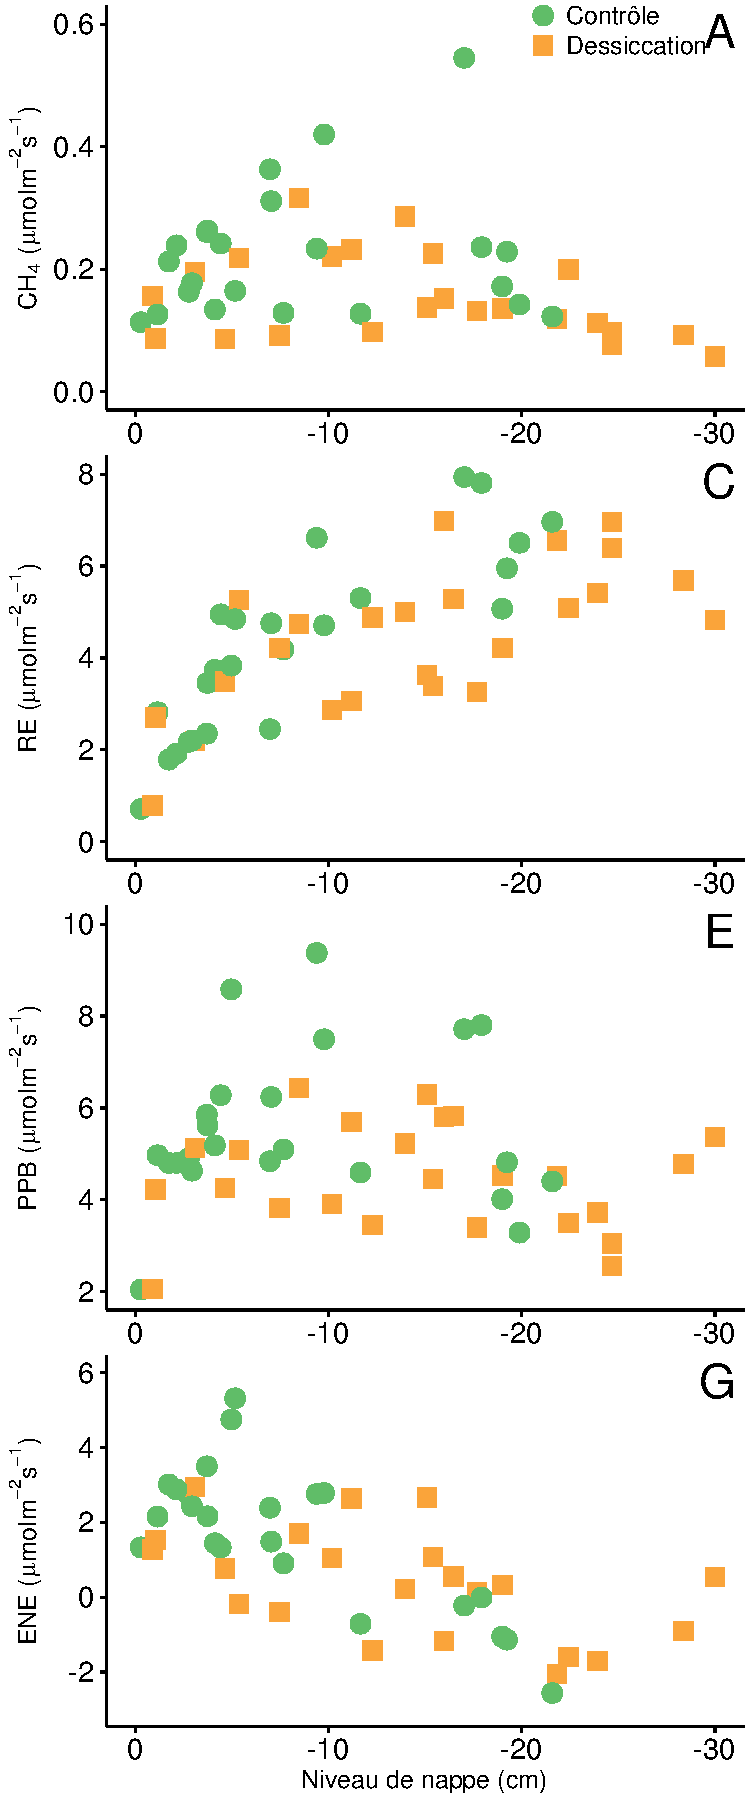
\includegraphics[width=\linewidth]{chap4/expA_fluxWTL}
\end{minipage}%
\begin{minipage}{.5\textwidth}
\centering
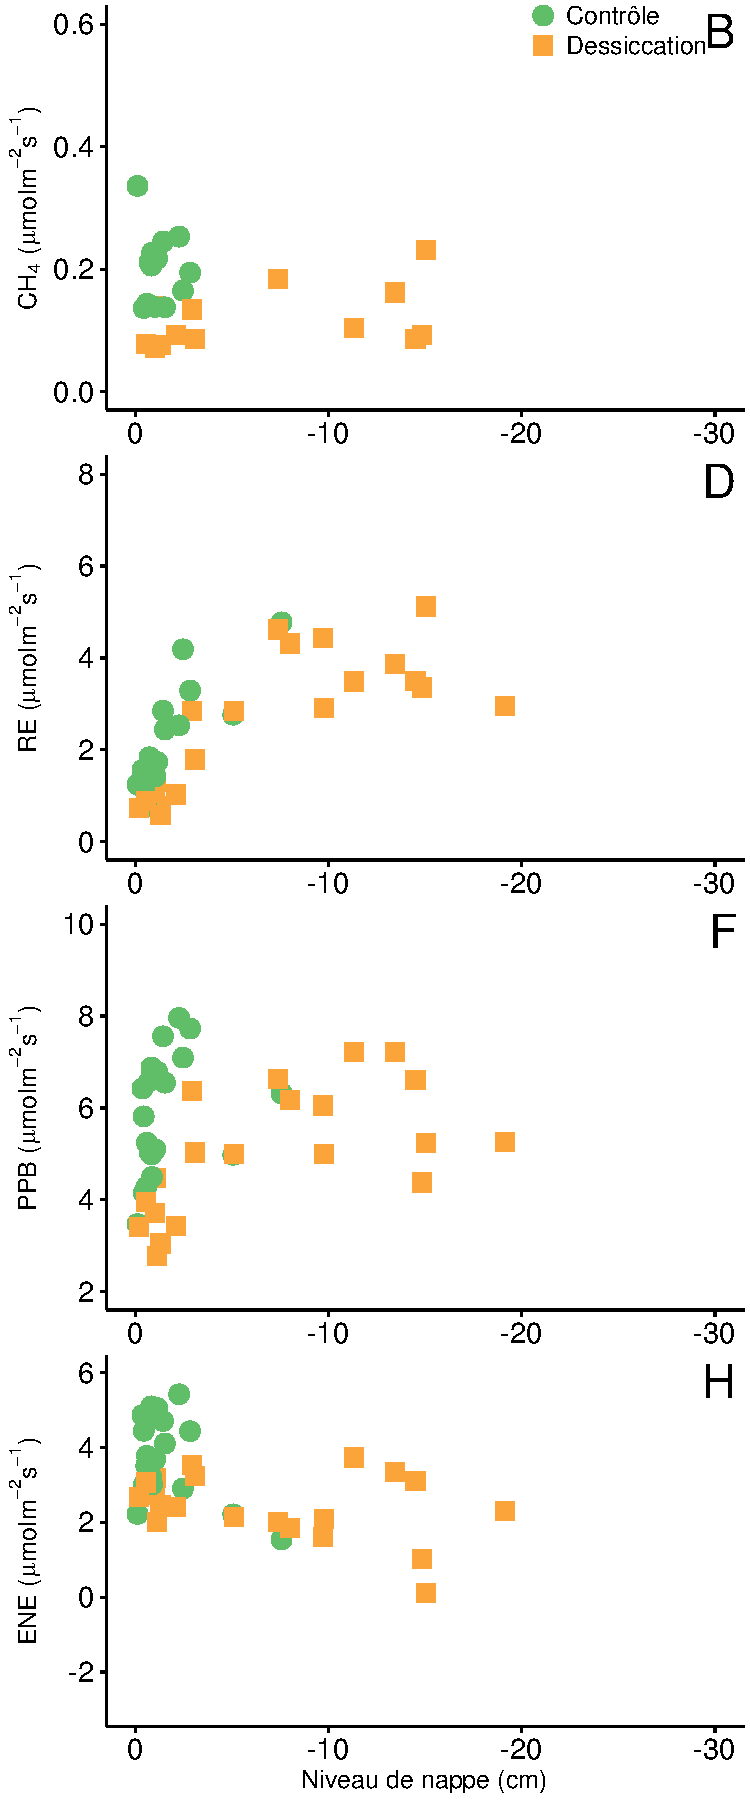
\includegraphics[width=\linewidth]{chap4/expB_fluxWTL}
\end{minipage}%
\caption{Relations entre les flux de GES, \chh (A et B), la RE (C et D), la PPB (E et F) et l'ENE (G et H), et le niveau de la nappe.}
\label{fig:hm_wtl}
\end{figure}

\begin{figure}[!tbp]
\centering
\hspace*{-2cm}
\begin{minipage}[]{.55\textwidth}
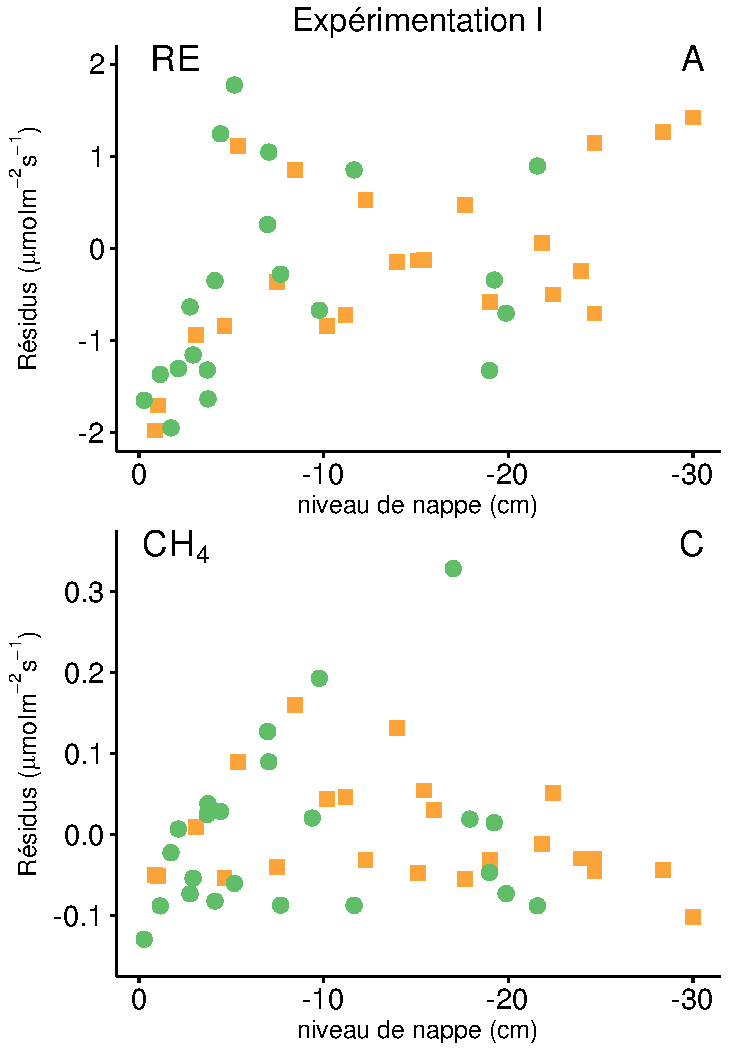
\includegraphics[width=\textwidth]{chap4/expA_res}
\end{minipage}
\hspace*{.1cm}
\begin{minipage}[]{.55\textwidth}
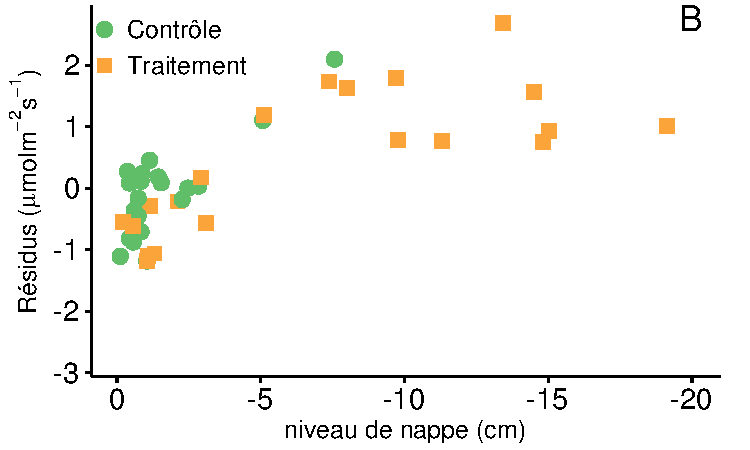
\includegraphics[width=\textwidth]{chap4/expB_res}
\end{minipage}
\hspace*{-2cm}
\caption{Relation entre les résidus d'équation du type $Flux=a*exp(b*Temp\acute{e}rature) $ reliant les flux de RE (A et B) et de \chh (C et D) au niveau de la nappe. La température de l'air est utilisée pour la RE des deux expérimentations (A et B), la température de la tourbe à \SI{-10}{\centi\metre} est utilisée pour l'expérimentation I et celle de la tourbe à \SI{-5}{\centi\metre} pour l'expérimentation II.}
\label{fig:HM_res}
\end{figure}


\subsection{Comparaison des deux expérimentations}

Pour le \chh, que ce soit pour l'expérimentation I ou B, aucune tendance ne semble se dégager vis à vis du niveau de la nappe (Figure~\ref{fig:hm_wtl}--A et B).
Une relation inverse est observée, pour les deux expérimentations, entre la RE et le niveau de la nappe (Figure~\ref{fig:hm_wtl}--C et D).
La PPB ne montre aucune tendance quelle que soit l'expérimentation.
Aux niveaux de nappe supérieurs à \SI{-20}{\centi\metre} de profondeur, correspondent des valeurs de PPB parmis les plus basses (Figure~\ref{fig:hm_wtl}--E).
%On peut noter que les valeurs de PPB les plus faibles correspondent aux niveaux de nappe les plus élevés (Figure~\ref{fig:hm_wtl}--E et F).
Pour les deux expérimentations, une relation est visible entre le niveau de la nappe et l'ENE qui diminue lorsque le niveau de nappe augmente (Figure~\ref{fig:hm_wtl}--G et H, expérimentation I : R\textsuperscript{2}=\num{0.52} ; p-value < \num{0.001} et  expérimentation II : R\textsuperscript{2}=\num{0.26} ; p-value < \num{0.001}).
Afin de séparer les effets de la température et ceux du niveau de la nappe, les résidus des équations reliant les flux à la température ont été calculés pour le \chh et la RE, qui semble contrôler en grande majorité les flux de \coo (Figure~\ref{fig:HM_res}).
La relation entre les résidus de la RE et le niveau de la nappe est moins claire une fois l'effet de la température retiré (Figure~\ref{fig:HM_res}, comparée à la Figure~\ref{fig:hm_wtl}--C).
Malgré tout, on peut observer une tendance à la hausse des résidus entre 0 et \SI{-18}{\centi\metre} pour les deux groupes de l'expérimentation I, puis une cassure, et à nouveau une tendance à la hausse pour le groupe « Dessiccation ».
Une tendance à augmenter des résidus de la RE quand le niveau de nappe diminue est également visible pour le groupe « Dessiccation » de l'expérimentation II (Figure~\ref{fig:HM_res}--B).
Cette hausse semble cependant s'amortir rapidement au delà de \SI{-10}{\centi\metre}.
Pour le \chh, aucune tendance entre les résidus de l'équation et le niveau de la nappe n'est visible pour l'expérimentation II (Figure~\ref{fig:HM_res}--D).
Pour l'expérimentation I, il est difficile d'observer une tendance claire même s'il semble y avoir un maximum des résidus liés au \chh autour de \SI{-10}{\centi\metre}(Figure~\ref{fig:HM_res}--C).


\section{Discussion}

\subsection{Comparaison des flux de carbone à ceux mesurés sur le terrain}
%CH4
\subsubsection{\chh}

Les flux moyens de \chh mesurés dans les mésocosmes des deux expérimentations sont parmi les valeurs hautes mesurées dans la tourbière de La Guette : certaines mesures dépassant le maximum de \SI{0.2}{\uml} que nous avons mesuré \textit{in-situ} en 2014.
Ces valeurs sont également dans la tranche haute des valeurs mesurées dans d'autres tourbières.
\citet{blodau2002}, dans un article de synthèse sur le cycle du carbone de plusieurs tourbières de l'hémisphère nord, montre que les flux de \chh varient généralement entre \num{0.004} et \SI{0.14}{\uml}.
Les valeurs mesurées restent cependant cohérentes avec celles observées par \citet{lai2014} dans une tourbière canadienne (\num{0}--\SI{0.56}{\uml}) ou par \citet{gogo2011} dans la tourbière de La Guette avec des flux compris entre \num{0.03} et \SI{0.4}{\uml} et mesurés en 2009.

\subsubsection{\coo}

Pour le \coo, les flux sont généralement dans la gamme des valeurs mesurées dans la tourbière de La Guette.
Pour l'expérimentation I, l'ENE moyen est plus faible que celui mesuré sur le terrain l'année 2013 : \num{0.81} contre \SI{2.85}{\uml}.
En revanche, pour l'expérimentation II, l'ENE moyen est de \SI{2.71}{\uml} ce qui est proche de celui mesuré sur le terrain : \SI{2.93}{\uml}.
Comme pour la RE, les flux de PPB sont du même ordre de grandeur que ceux mesurés sur le terrain, mais dans la gamme basse : les maximas moyens mesurés dans les mésocosmes sont d'environ \num{7.5} pour des valeurs de \SI{13}{\uml} mesurées dans la tourbière.
Ces valeurs restent cohérentes avec la littérature (e.g. \citealp{bortoluzzi2006a}).

%
%Les flux de RE et de PPB sont moins élevés que ceux mesurés sur le terrain mais restent dans la même gamme de valeurs.
%Ces comparaisons sont par ailleurs à relativiser puisque les mesures de flux n'ont pas nécessairement lieu aux mêmes moments de la journée.



\subsection{Effet des variations du niveau de la nappe sur les flux de gaz}

\subsubsection{\chh}
%Si les flux de \chh sont liés aux températures, notamment 
Les flux de \chh sont plus élevés pendant les phases de dessiccation que lors des phases de réhumectation.
Cette observation va à l'encontre de l'hypothèse qui stipule qu'une baisse du niveau de la nappe fait baisser les flux de \chh, en augmentant la zone propice à son oxydation et en diminuant la zone propice à sa production \citep{aerts1997,pelletier2007,turetsky2008}.
\citet{kettunen1996}, dans une étude \textit{in-situ}, rapportent eux aussi une relation inverse entre les flux de \chh et le niveau de la nappe.
Ils expliquent cette observation par le fait qu'une baisse du niveau de la nappe peut permettre une libération du méthane accumulé dans une porosité précédemment scellée par la saturation en eau.
Des observations similaires sont rapportées par \citet{bellisario1999}, sur une tourbière où le niveau de la nappe d'eau varie entre \num{-1} et \SI{-13}{\centi\metre}, et par \citet{treat2007} où le niveau de nappe varie entre \num{-9} et \SI{-30}{\centi\metre}.
Ces derniers expliquent également l'augmentation des flux de \chh, suite à une baisse du niveau de la nappe, par une diminution de la pression de l'eau qui libère du \chh auparavant bloqué dans une porosité isolée de l'atmosphère.
Le point commun de ces travaux est un niveau de nappe relativement élevé, majoritairement supérieur à \SI{-30}{\centi\metre}.
%Ce niveau de nappe élevé semble permettre au phénomène de transport du \chh de prendre le pas, sur les phénomènes de production/oxydation qui sont traditionnellement liés aux fluctuations du niveau de l'eau.
Un niveau de nappe élevé semble influencer les émissions de \chh plus par son action sur le transport de ce gaz que sur le rapport production/oxydation du \chh.
Autrement dit, dans cette gamme de variation du niveau de la nappe d'eau (0, \SI{-20}{\centi\metre}), les variations de flux de \chh observées seraient davantage liées à des effets de pression de l'eau, ouvrant ou fermant une partie de la porosité du sol et permettant ou empêchant le transport de \chh.

Cette hypothèse permet d'expliquer, pour l'expérimentation II, le pic de \chh observé lors du passage de R1 à D2 (Groupe « Dessiccation », Figure~\ref{fig:HMzi}).
La baisse d'émission de \chh observée entre D3 et R3 s'expliquerait alors par un blocage du transport lié à la réhumectation.

Le fait que les groupes « Dessiccation », quelle que soit la phase et l'expérimentation, aient des flux de \chh plus faibles que les groupes « Contrôle » peut s'expliquer par le fait que les micro-organismes méthanogènes soient peu perturbés par les dessiccations dans les groupes « Contrôle » par rapport aux groupes « Dessiccation ».
Ceci est en cohérence avec les études montrant un effet positif de la présence d'eau sur les flux de \chh.
La production de \chh des groupes « Contrôle » est donc plus forte que celles des groupes « Dessiccation ».
De plus, après le premier abaissement du niveau de la nappe, une partie de la communauté des méthanogènes est probablement non active ou a migré dans le bas de la colonne de tourbe.
La production des groupes « Dessiccation » est donc localisée plus bas que celle des groupes « Contrôle ».

Ceci semble cohérent avec les observations faites pendant l'expérimentation I.
En effet malgré une dessiccation du groupe « Contrôle » pendant le mois de juin (baisse de la teneur en eau du sol), ce dernier est beaucoup plus réactif que le groupe « Dessiccation » lors de l'augmentation de température qui a lieu à partir de début juillet.
On peut faire l'hypothèse que les événements pluvieux subis par le groupe « Contrôle » lui ont permis de maintenir une communauté active de méthanogènes plus longtemps.
Avant la réhumectation les deux groupes ont des flux de \chh similaires, ils semblent donc avoir atteint un niveau d'assèchement proche.
L'état de leurs méthanogènes respectifs devrait également être similaire.
Pendant la réhumectation les méthanogènes se réactivent, mais les flux sont bloqués par la saturation en eau, le \chh est émis avec un retard lorsque le niveau d'eau diminue.

Il ressort de ces deux expérimentations qu'un niveau de nappe élevé favorise, sur le long terme, les émissions de \chh, mais d'autres effets peuvent interférer localement et notamment le bloquage ponctuel du transport de \chh par un niveau de nappe proche ou à la surface du sol.
Le \chh peut ensuite être émis lorsque le niveau de la nappe d'eau diminue.
Ces écarts temporels qui peuvent exister entre la production et l'émission du \chh rendent difficile d'établir une relation directe entre les flux de \chh et ses facteurs de contrôle, que ce soit la température ou le niveau de la nappe.

%En outre, la réhumectation peut bloquer le transport de cette production.
%Cet écart temporel entre la production et l'émission de \chh, lié à ce phénomène, rend difficile d'établir une relation directe entre le \chh et les variables qui contrôlent sa production, que ce soit la température ou le niveau de la nappe.
% TO WRITE !!!!!!!!!!!!! ok cf ci dessus
%Pourquoi ch4 dess tjs < ch4 ctrl ? D1 >> (libération ch4) destruction, migration de la comm ana, ensuite R (production mais transport bloqué), D2, libération du ch4 produit pdt D1...
%Alors que pour ctrl la communauté et tjs en place sur l'ensemble de la colonne (production > à trt), (évolution // à la PPB ?)

\subsubsection{\coo}

Dans les deux expérimentations, une baisse du niveau de la nappe conduit à une augmentation de la RE, ce qui est en accord avec la littérature, que ce soit des expérimentations en mésocosmes \citet{blodau2004,dinsmore2009} ou sur le terrain \citet{ballantyne2014}. 

Pour l'expérimentation I, cette augmentation de la RE conduit à une baisse de l'ENE pendant la première phase de dessiccation.
Pendant la phase de réhumectation les flux de RE diminuent.
Après la phase de dessiccation les flux de RE retrouvent la même intensité qu'avant la réhumectation.
Dans le même temps la PPB augmente et empêche l'ENE de décroître à nouveau.
La PPB du groupe « Contrôle » est supérieure à celle du groupe « Dessiccation ».
La dessiccation du groupe « Dessiccation » a davantage atteint la végétation que celle du groupe « Contrôle ».


Globalement, dans les deux expérimentations, l'ENE est plus faible dans les groupes « Dessiccation » que dans les groupes « Contrôle » ce qui est en accord avec la littérature (Tableau~\ref{table:bib_wtl})
%L'expérimentation II montre bien que la baisse du niveau de la nappe fait augmenter la RE.
%Les pics de RE observés pour le groupe « Contrôle » sont systématiquement liée à une légère diminution du niveau de la nappe d'eau (campagnes n°5, 11, 17 et 18).
%La forte intensité de ces flux, par rapport à la variation du niveau de la nappe d'eau suggère que des effets sur le transport peuvent intervenir.
%L'augmentation de l'ENE sur l'ensemble de l'expérimentation va à l'encontre de ce qui est généralement observé (Tableau~\ref{table:bib_wtl}.).
%Pour expliquer cette tendance on peut faire l'hypothèse que les conditions de saturation en eau particulièrement importantes ont impactées les communautés de micro-organismes aérobies.
%Des variations de nappes plus importantes auraient peut-être changé cette tendance.
%En effet dans \citet{blodau2004} et \citet{dinsmore2009} par exemple, les mésocosmes utilisés sont plus grands, 75 et \SI{41}{\centi\metre} de hauteur respectivement, ont permis d'abaisser le niveau de l'eau en dessous de \SI{-30}{\centi\metre}.
%Cette limite a été rapportée plusieurs fois comme étant un seuil au delà duquel sont observés des changements importants \citep{blodau2004,peichl2014}.
%Ce seuil serait également une limite au delà de laquelle les forces de capillarité ne permettraient plus d'alimenter en eau les sphaignes \citep{rydin2013a,ketcheson2014}.

%Pour les deux expérimentations, les valeurs de l'ENE sont proches avant la première phase de dessiccation.
%À partir de cette dernière, l'ENE des groupes « Dessiccation » est systématiquement plus faible que celui des groupes « Contrôle ».
%L'observation de valeurs d'ENE plus faibles pour un niveau de nappe plus bas est cohérente avec la littérature, que ce soit des expérimentations en mésocosmes \citet{aerts1997,blodau2004} ou sur le terrain \citet{bubier2003,sonnentag2010}.
%
%Pour l'expérimentation I, la cause de cette baisse de l'ENE semble d'abord être une RE plus forte pour le groupe Dessication que pour le groupe « Contrôle » pendant les campagnes n°3 à 9.
%Par la suite, entre les deux groupes, la différence de RE est moins importante, voire s'inverse, et les deux groupes se retrouvent avec un ENE similaire.
%Après la phase de réhumectation, à partir de la campagne n°20, la différence de valeurs de l'ENE entre les deux groupes est à nouveau présente et semble cette fois s'expliquer davantage par la PPB (plus forte pour le groupe « Contrôle ») que par la RE. (\textbf{justif photo sphaigne ?}).
%Pour l'expérimentation II, la différence entre l'ENE du groupe « Contrôle » et celui du groupe « Dessiccation » est lié à une RE plus importante pendant les phases de dessiccation et à une PPB plus faible pendant les phases de réhumectation.
%
%Dans les deux expérimentations, une baisse du niveau de la nappe conduit à une augmentation de la RE, ce qui est en accord avec la littérature, que ce soit des expérimentations en mésocosmes \citet{blodau2004,dinsmore2009} ou sur le terrain \citet{ballantyne2014}. 
%L'effet de la baisse du niveau de la nappe sur la PPB semble être au contraire limité que ce soit pour l'expérimentation I ou II.
%La taille des mésocosmes et l'amplitude des variations de la nappe sont peut-être assez importantes.
%En effet dans \citet{blodau2004} et \citet{dinsmore2009} par exemple, les mésocosmes utilisés sont plus grands, 75 et \SI{41}{\centi\metre} de hauteur respectivement, ont permis d'abaisser le niveau de l'eau en dessous de \SI{-30}{\centi\metre}.
%Cette limite a été rapportée plusieurs fois comme étant un seuil au delà duquel sont observés des changements importants \citep{blodau2004,peichl2014}.
%Ce seuil serait également une limite au delà de laquelle les forces de capillarité ne permettraient plus d'alimenter en eau les sphaignes \citep{rydin2013a,ketcheson2014}.

%Les résultats de ces deux expérimentations montrent une augmentation de la RE quand le niveau de la nappe diminue.
%Ceci est en accord avec les résultats d'autres études que ce soit in-situ \citep{ballantyne2014} ou en mésocosmes \citep{blodau2004,dinsmore2009}.
%Dans ces deux dernières publications, la baisse du niveau de la nappe diminue la PPB.
%Pas de variations significatives de la PPB avec le niveau de la nappe n'est visible dans les données présentées, même si une légère tendance semble émergée aux plus fortes profondeur de nappe pour l'expérimentation I.
%Cette absence d'effet du niveau de la nappe sur la PPB peut, être liée à la profondeur des mésocosmes (\SI{30}{\centi\metre}).
%En effet dans \citet{blodau2004} et \citet{dinsmore2009}, les mésocosmes utilisés sont plus grands, 75 et \SI{41}{\centi\metre} respectivement, ont permis d'abaisser le niveau de l'eau au delà de \SI{-30}{\centi\metre}.
%Cette limite a été rapportée plusieurs fois comme étant un seuil au delà duquel son observés des changements importants \citep{blodau2004,peichl2014}.
%Ce seuil est expliqué comme étant la limite au delà de laquelle les forces de capillarités ne permettent plus d'alimenter en eau les sphaignes \citep{rydin2013a,ketcheson2014}.
%Il résulte des constats précédents qu'une baisse du niveau de nappe, faisant augmenter la RE et ne changeant pas ou peu la PPB, conduit à une baisse de l'ENE.
%Cette diminution de l'ENE est cohérente avec la littérature, que ce soit des expérimentations en mésocosmes \citep{aerts1997,blodau2004}, ou in-situ \citep{bubier2003,sonnentag2010}.
%Malgré tout l'extrapolation de ses résultats à d'autres situations n'est pas aisée car fortement fonction du contexte.
%D'autre études n'ont, par exemple, pas observé d'influence du niveau de la nappe sur la RE \citep{updegraff2001}.
%Par ailleurs \citet{laiho2006} a montré l'importance du contexte et notamment celui de l'échelle de temps considéré qui peut impliquer des phénomènes différents et donc avoir des conséquences différentes.

%La dépendance entre les flux de \chh et le niveau de la nappe, devant conduire à une baisse des émissions quand le niveau de la nappe diminue, comme décrite dans \citet{aerts1997}, \citet{pelletier2007} ou \citet{turetsky2008}, n'a pas été clairement observée.
%Ce constat rejoins d'autres études dans lesquelles une relation inverse ou un absence de relation a été trouvé entre le \chh et le niveau de la nappe \citet{kettunen1996,bellisario1999,treat2007}.
%L'observation d'un pic de méthane suivant de quelques jours une phase de hausse du niveau de la nappe, est également rapportée par \citet{kettunen1996}. \textbf{(And so what ?)}


%\subsection{Dessication}
%
%Lors des phases de dessiccations, les deux expérimentations montrent une hausse de la RE, que l'assèchement soit sur une période longue (expérimentation I) ou plus courte (expérimentation II).
%À cause des conditions météorologiques présentes lors de l'expérimentation I, le groupe de contrôle subit également un assèchement et donc une hausse de sa RE.
%À l'inverse les conditions météorologique moins ensoleillée de l'expérimentation II ont permis d'observer une différence nette entre d'assèchement du groupe traité et celui du groupe de contrôle.
%Pour cette expérimentation, la différence entre la RE des deux groupes est statistiquement différente (p<0.05) pendant les phases de dessiccation mais non pendant les phases de réhumectation.
%À l'exception du cycle 3 pour lequel la différence entre traitement et contrôle est également significative.
%La RE est donc impactée de façon significative lors d'un assèchement et même si les différences ne sont significative que pour R3, il est intéressant de noter que pendant les phases de réhumectation la RE du groupe traité tend à être plus faible que celle du groupe de contrôle.
%Ainsi les cycles de dessiccation/réhumectation semblent augmenter les extrêmes de la gamme de valeur de la RE.
%
%La baisse du \chh observé dans l'expérimentation I, 
%
%
%Discuter les hausses de CH4 et de RE à partir du 23 juin pour Zi.
%
%\subsection{Réhumectation}
%
%La réhumectation après une phase de dessiccation fait baisser la RE, que ce soit pour l'expérimentation I ou l'expérimentation II.
%
%Il semble y avoir une émission de \chh suite aux phases de réhumectation, mais avec un certain temps de latence.
%L'expérimentation I le montre  de façon relativement clair.
%Par contre si des pics sont également visible dans l'expérimentation II, la faible durée des cycles ne permet pas de déterminer s'ils sont liés à la réhumectation ou à la phase de dessiccation qui suit.

\subsection{Effet des cycles hydrologiques multiples sur les flux de GES}

La multiplicité des cycles de l'expérimentation II semble montrer que la différence entre l'ENE observée dans les deux groupes, pendant les phases de réhumectation, tend à augmenter avec le temps.
Ce qui indiquerait une baisse de la résilience de l'écosystème après les événements de dessiccation.
Cependant davantage de points de mesures par cycle semble nécessaires pour établir un lien significatif entre fréquence des dessiccations et résilience du système.


\subsection{Conclusions}

Les deux expérimentations ont montré que malgré des dynamiques différentes, une baisse du niveau de la nappe d'eau conduisait à une augmentation de la RE et qu'un niveau de nappe haut favorisait les émissions de \chh.
Mais elles ont également mis en évidence que d'autres phénomènes interférent.
Notamment le blocage des flux par une saturation en eau élevée peut conduire à observer des émissions qui semblent contradictoires à celles que l'on attendrait (moins d'émissions de \chh quand le niveau de nappe est le plus élevé).
Au delà de la valeur absolue du niveau de la nappe, l'histoire et l'intensité de ses variations peut donc jouer un rôle important sur les flux de GES mesurés.